\documentclass[a4paper,12pt]{report}
\usepackage{a4wide}

%\documentclass[a5paper,10pt]{book}
%\usepackage[top=23mm, bottom=18mm, left=15mm, right=25mm]{geometry}
%\geometry{papersize={170mm,220mm}}


\usepackage[utf8x]{inputenc}
\usepackage[danish]{babel}

\usepackage{xr-hyper} %Externe hyper-ref
\usepackage[colorlinks=true, hyperindex=true, linkcolor=minmblaa, citecolor=minmblaa, urlcolor=minmblaa]{hyperref}
\hypersetup{colorlinks=true,filecolor=minmblaa,bookmarksnumbered=true} %Til hyperreferencer. Referencer med farver
\usepackage{needspace} % giver mulighed for at kræve at der skal være et antal tomme linier på siden før ellers indsættes et sideskift.
\usepackage{framed} %Bokse
\usepackage{wrapfig}

\usepackage{amsmath,amsfonts,amssymb,amsthm,mathtools} %Matematikpakker

\setlength{\parindent}{0mm} %Ingen Indhak i første linje i afsnit

\usepackage{color} %Farvepakke

\usepackage{array}
\usepackage{colortbl}
\usepackage{multirow} %Til at flette rækker i tabeller.

\usepackage{verbatim,mhchem}



	% DOWNLOAD FRA: http://sarovar.org/frs/?group_id=52&release_id=97
	% Læg i directory for hoved TEX fil
%\usepackage[draft]{pdfdraftcopy}
%\draftstring{Licens: Kasper Langt Mellemnavn Skårhøj}
%\draftfontsize{30}
	%\draftfontfamily{hlh}
	%\draftangle{45}
	%\definecolor{mycolor}{rgb}{.825,.855,1}
	%\draftcolor{mycolor}
	%\draftfontattrib



% = Sidehoved =
\usepackage{fancyhdr}
\pagestyle{fancy}
\renewcommand{\sectionmark}[1]{\markright{\protect\titlegraphic{dturoed}\textcolor{dtugraa}{\thesection~\MakeUppercase{#1}}}} % \thesection.\
\fancyhead{}
\fancyfoot{}
\fancyhead[R]{\titlefont\thepage}
\fancyhead[C]{}
\fancyhead[L]{\titlefont \small eNote \MakeUppercase{~\thechapter}~\hspace*{1ex}\rightmark}
\renewcommand\headrulewidth{0pt}
\fancypagestyle{plain}{\fancyfoot[C]{}}% {\titlefont\footnotesize\thepage}}
\setlength{\headheight}{15pt}


% = Længder
%\newlength{\envtblsep}\setlength{\envtblsep}{1\FrameSep}
\newlength{\obsl}\setlength{\obsl}{\textwidth-1.2cm-13.2pt}

% Includes:

% =     Fonts (select one)    =
\usepackage{mathpazo}\linespread{1.05} % Palatino needs more leading (space between lines)
\usepackage{bm} % bold math, must be loaded after the fontpackages

% % Til overskrifter
\DeclareTextFontCommand{\th}{\fontencoding{T1}\fontfamily{phv}\fontseries{b}\selectfont}
\newcommand\titlefont{\fontencoding{T1}\fontfamily{phv}\selectfont}


% =     PGF grafik      =
\usepackage{tikz}
\newcommand\titlegraphic[1]{%
\tikz[baseline] %
\draw[thick,color=#1]
(0pt  ,-0.25em) -- (0pt  ,0.85em)
(2.5pt,-0.25em) -- (2.5pt,0.85em)
(5pt  ,-0.25em) -- (5pt  ,0.85em)
(7.5pt,-0.25em) -- (7.5pt,0.85em);\hspace*{0.8ex} %
}

\newcommand\titlegraphicwide[1]{%
\tikz[baseline] %
\draw[line width=0.8mm,color=#1]
(0pt  ,-0.25em) -- (0pt  ,0.85em)
(4.5pt,-0.25em) -- (4.5pt,0.85em)
(9pt  ,-0.25em) -- (9pt  ,0.85em)
(13.5pt,-0.25em) -- (13.5pt,0.85em);\hspace*{0.8ex} %
}


% =      Title Layout      =
\usepackage{titlesec}
\makeatletter
\titleformat{\chapter}
	[display] % Shape
	{\titlefont\Huge\flushleft} % Title and label format
	{\titlefont\LARGE\bfseries \titlegraphicwide{dturoed}\textcolor{dtugraa}{\@chapapp~\thechapter}} % label
	{0.9em} % label/title separation
	{} % before code
	[] % after code
\makeatother
\titleformat{\section}
	[hang] % Shape
	{\titlefont\Large\flushleft} % Title and label format
	{\thesection} % label
	{0.9em} % label/title separation
	{} % before code
	[] % after code
\titleformat{\subsection}
	[hang] % Shape
	{\titlefont\large} % Title and label format
	{\thesubsection} % label
	{0.9em} % label/title separation
	{} % before code
	[] % after code
\titlespacing{\subsection}{0pt}{*6}{*1.5}
\titleformat{\subsubsection}
	[hang] % Shape
	{\titlefont} % Title and label format
	{\thesubsubsection} % label
	{0.9em} % label/title separation
	{} % before code
	[] % after code



% = Farver
\definecolor{dturoed}{rgb}{0.6, 0.0, 0.0}
\definecolor{dtugraa}{rgb}{0.5, 0.5, 0.5}	% Lidt mørkere. Korrekt = 0.4
\definecolor{mingroenstreg}{rgb}{0.4,0.8,0}	% Sekundærfarve 14 : 102/204/0	(Forårsgrøn) -> Eksempler
\definecolor{mingroen}{rgb}{0.32,0.64,0}		% Sekundærfarve 14, 80% mørkere (tekst)
\definecolor{minorangestreg}{rgb}{1,0.6,0}		% Sekundærfarve 1 : 255/153/0	(Orange) -> Opgaver
\definecolor{minorange}{rgb}{0.8,0.48,0}		% Sekundærfarve 1 , 80% mørkere (tekst)

\definecolor{minblaa}{rgb}{0.2,0.4,0.8}	% Sekundærfarve 13 , 51/102/204 	( Blå -> Definitioner etc)
\definecolor{minmblaa}{rgb}{0.16,0.32,0.64}	% Sekundærfarve 13 , 80% mørkere (tekst)
\definecolor{thmbackground}{rgb}{0.97,.97, 0.99}	% Farve 13 - lys baggrund

\definecolor{mingraastreg}{rgb}{.5,.5,.5}
\definecolor{hvadbackground}{rgb}{0.97,.97, 0.97}
\definecolor{sumgul}{rgb}{1,1,.8}

\definecolor{hjmopgfarve}{rgb}{.96,1,.96}


% = Counter
\newcounter{evncount}[chapter]
\setcounter{evncount}{0}
\renewcommand{\theevncount}{\thechapter.\arabic{evncount}}
\renewcommand{\theequation}{\thechapter-\arabic{equation}}


% = Eksempler = example =
\newenvironment{example}[1][]{
	\refstepcounter{evncount}
	\setlength{\obsl}{\textwidth-1.2cm-13.2pt-9pt} % fix width of the info envirnment%
	\def\FrameCommand{ 
		\textcolor{mingroenstreg}{\vrule width 4pt} 
		\hspace{5pt} 
	}%
	\MakeFramed{\advance\hsize-\width \FrameRestore}%
	\needspace{3\baselineskip}
	\titlegraphic{mingroen}
	\textcolor{mingroen}{
		\th{Eksempel \theevncount \hspace*{5mm} #1}
	} 
	\vspace*{3mm}%
	\begin{small}
	\par
}
{
	\end{small}
	\endMakeFramed
}


% = Opgaver = exercise =
\newenvironment{exercise}[1][]{
	\refstepcounter{evncount}
	\setlength{\obsl}{\textwidth-1.2cm-13.2pt-9pt}% fix width of the info envirnment%
	\def\FrameCommand{
		\textcolor{minorangestreg}{\vrule width 4pt}
		\hspace{5pt}
	}%
	\MakeFramed{\advance\hsize-\width \FrameRestore}%
	\needspace{3\baselineskip}
	\titlegraphic{minorange}
	\textcolor{minorange}{
		\th{Opgave \theevncount \hspace*{5mm} #1}
	} 
	\vspace*{3mm}%
	\begin{small}
	\par
}
{
	\end{small}
	\endMakeFramed
}


% = Bevis
\newenvironment{bevis}{
	\setlength{\obsl}{\textwidth-1.2cm-13.2pt-9pt} % fix width of the info envirnment%
	\def\FrameCommand{
		\textcolor{mingraastreg}{\vrule width 4pt} 
		\hspace{5pt}
	}%
	\MakeFramed{\advance\hsize-\width \FrameRestore}%
	\needspace{3\baselineskip}
	\titlegraphic{black}
	\textcolor{black}{
		\th{Bevis}
	}
	\vspace*{3mm}%
	\begin{small}
	\par
}
{
	\bevisslut 
	\end{small}
	\endMakeFramed
}


% = Definition =
\newenvironment{definition}[1][]{
	\vspace{4mm}
	\pagebreak[1]
	\setlength{\obsl}{\textwidth-1.2cm-2\FrameSep-13.2pt}%
	\def\FrameCommand{
		\fboxsep=\FrameSep\fcolorbox{minblaa}{thmbackground}
	}
	\begin{minipage}{\textwidth}
	\MakeFramed{\advance\hsize-\width\FrameRestore}
	\refstepcounter{evncount}
	\titlegraphic{minblaa}
	\textcolor{minmblaa}{
		\th{Definition \theevncount \hspace*{5mm} #1}
	}
	\vspace*{3mm}
	\par
}
{
	\endMakeFramed 
	\end{minipage}
	\vspace{4mm}
}


% = Theorem =
\newenvironment{theorem}[1][]{
	\vspace{4mm}
	\pagebreak[1]%
	\setlength{\obsl}{\textwidth-1.2cm-2\FrameSep-13.2pt}%
	\def\FrameCommand{
		\fboxsep=\FrameSep\fcolorbox{minblaa}{thmbackground}
	}%
	\begin{minipage}{\textwidth}
	\MakeFramed{\advance\hsize-\width\FrameRestore}%
	\refstepcounter{evncount}
	\titlegraphic{minblaa}
	\textcolor{minmblaa}{
		\th{Sætning \theevncount \hspace*{5mm} #1}
	}
	\vspace*{3mm}
	\par
}
{
	\endMakeFramed 
	\end{minipage}
	\vspace{4mm}
}


% = Lemma =
\newenvironment{lemma}[1][]{
	\vspace{4mm}
	\pagebreak[1]
	\setlength{\obsl}{\textwidth-1.2cm-2\FrameSep-13.2pt}%
	\def\FrameCommand{
		\fboxsep=\FrameSep \fcolorbox{minblaa}{thmbackground}
	}
	\begin{minipage}{\textwidth} 
	\MakeFramed{\advance\hsize-\width \FrameRestore}
	\refstepcounter{evncount}
	\titlegraphic{minblaa}
	\textcolor{minmblaa}{
		\th{Hjælpesætning \theevncount \hspace*{5mm} #1}
	}
	\vspace*{3mm}
	\par
}
{
	\endMakeFramed 
	\end{minipage}
	\vspace{4mm}
}


% = Corollary =
\newenvironment{corollary}[1][]{
	\vspace{4mm}
	\pagebreak[1]
	\setlength{\obsl}{\textwidth-1.2cm-2\FrameSep-13.2pt}%
	\def\FrameCommand{
		\fboxsep=\FrameSep \fcolorbox{minblaa}{thmbackground}
	}
	\begin{minipage}{\textwidth} 
	\MakeFramed{\advance\hsize-\width \FrameRestore}
	\refstepcounter{evncount}
	\titlegraphic{minblaa}
	\textcolor{minmblaa}{
		\th{Følgesætning \theevncount \hspace*{5mm} #1}
	}
	\vspace*{3mm}
	\par
}
{
	\endMakeFramed 
	\end{minipage}
	\vspace{4mm}
}


% = Metode = method
\newenvironment{method}[1][]{
	\vspace{4mm}
	\pagebreak[1]
	\setlength{\obsl}{\textwidth-1.2cm-2\FrameSep-13.2pt}%
	\def\FrameCommand{
		\fboxsep=\FrameSep \fcolorbox{black}{hvadbackground}
	}
	\begin{minipage}{\textwidth} 
	\MakeFramed{\advance\hsize-\width \FrameRestore}
	\refstepcounter{evncount}
	\titlegraphic{black}
	\textcolor{black}{
		\th{Metode \theevncount \hspace*{5mm} #1}
	}
	\vspace*{3mm}
	\par
}
{
	\endMakeFramed
	\end{minipage}
	\vspace{4mm}
}


% = Forklaring = explain =
\newenvironment{explain}[1][]{
	\vspace{4mm}
	\pagebreak[1]
	\setlength{\obsl}{\textwidth-1.2cm-2\FrameSep-13.2pt}%
	\def\FrameCommand{
		\fboxsep=\FrameSep \fcolorbox{black}{hvadbackground}
	}
	\MakeFramed{\advance\hsize-\width \FrameRestore}
	\refstepcounter{evncount}
	\titlegraphic{black}
	\textcolor{black}{
		\th{Forklaring \theevncount \hspace*{5mm} #1}
	}
	\vspace*{3mm}
	\par
}
{
	\endMakeFramed
	\vspace{4mm}
}


% = Bemærkning = remark =
\newenvironment{remark}[1][]{
	\vspace{4mm}
	\pagebreak[1]
	\setlength{\obsl}{\textwidth-1.2cm-2\FrameSep-13.2pt}%
	\def\FrameCommand{
		\fboxsep=\FrameSep \fcolorbox{black}{hvadbackground}
	}
	\begin{minipage}{\textwidth} 
	\MakeFramed{\advance\hsize-\width \FrameRestore}
	\refstepcounter{evncount}
	\titlegraphic{black}
	\textcolor{black}{
		\th{Bemærkning \theevncount \hspace*{5mm} #1}
	}
	\vspace*{3mm}
	\par
}
{
	\endMakeFramed 
	\end{minipage}
	\vspace{4mm}
}







% = OBS! = obs =
\newenvironment{obs}{\vspace{4mm}\par%
\begin{tabular}{m{1.2cm}<{\hspace*{2mm}}@{}|m{\obsl}@{}}\hspace*{-4pt}\raggedleft
\includegraphics[width=1.1cm]{../Strukturfiler/FIGS/Alert01} & \begin{minipage}{\obsl}}{\end{minipage}\\ \end{tabular}\vspace{4mm}\par}


% = INFO = info =
\newenvironment{info}{\vspace{4mm}\par%
\begin{tabular}{m{1.2cm}<{\hspace*{2mm}}@{}|m{\obsl}@{}}\hspace*{-4pt}\raggedleft
\includegraphics[width=1.1cm]{../Strukturfiler/FIGS/Info01} & \begin{minipage}{\obsl}}{\end{minipage}\\ \end{tabular}\vspace{4mm}\par}


% = THINK= think =
\newenvironment{think}{\vspace{4mm}\par%
\begin{tabular}{m{1.2cm}<{\hspace*{2mm}}@{}|m{\obsl}@{}}\hspace*{-4pt}\raggedleft
\includegraphics[width=0.7cm]{../Strukturfiler/FIGS/ChessPiece} & \begin{minipage}{\obsl}}{\end{minipage}\\ \end{tabular}\vspace{4mm}\par}


% = AHA= aha =
\newenvironment{aha}{\vspace{4mm}\par%
\begin{tabular}{m{1.2cm}<{\hspace*{2mm}}@{}|m{\obsl}@{}}\hspace*{-4pt}\raggedleft
\includegraphics[width=1.1cm]{../Strukturfiler/FIGS/Think} & \begin{minipage}{\obsl}}{\end{minipage}\\ \end{tabular}\vspace{4mm}\par}


% = BUILDUP= build =
\newenvironment{build}{\vspace{4mm}\par%
\begin{tabular}{m{1.2cm}<{\hspace*{2mm}}@{}|m{\obsl}@{}}\hspace*{-4pt}\raggedleft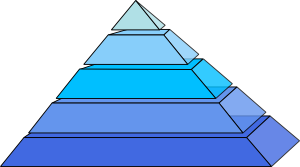
\includegraphics[width=1.1cm]{../Strukturfiler/FIGS/BluePyramid} & \begin{minipage}{\obsl}}{\end{minipage}\\ \end{tabular}\vspace{4mm}\newline}


% = Forudsætning = basis
\newenvironment{basis}{\begin{flushleft} \begin{itshape} }{\end{itshape} \end{flushleft}}


% = Opsummering =
\newenvironment{summary}{\clearpage\pagecolor{sumgul}\section{Opsummering}}{\newpage\pagecolor{white}}











% = Counter
\newcounter{opgavecount}[section]
\setcounter{opgavecount}{0}
\newcounter{spgcount}[opgavecount]
\setcounter{spgcount}{0}
\renewcommand{\thespgcount}{\alph{spgcount})}



% = EXERCISE = (DIVIDER)

\newcommand{\exercisebegin}[1][]{\bigskip\needspace{3\baselineskip}\refstepcounter{opgavecount}\titlegraphic{mingroen}\textcolor{mingroen}{\th{Opgave \theopgavecount \hspace*{1cm} #1}}\medskip\par}

% = QUIZEXERCISE = (DIVIDER)

\newcommand{\quizexercisebegin}[1][]{\bigskip\needspace{3\baselineskip}\refstepcounter{opgavecount}\titlegraphic{mingroen}\textcolor{mingroen}{\th{Quiz-Opgave \theopgavecount \hspace*{1cm} #1}}\medskip\par}

% = QUESTION =

\newenvironment{question}{\refstepcounter{spgcount}\begin{itemize}\item[\thespgcount]}{\end{itemize}\hspace*{\fill}}

% = VINK =

\newenvironment{vink}{\begin{tabular}{m{.9cm}<{\hspace*{2mm}}@{}|m{\obsl}@{}}\hspace*{-4pt}\raggedleft
\includegraphics[width=.9cm]{../Strukturfiler/FIGS/Think} & \begin{minipage}{\obsl}}{\end{minipage}\\ \end{tabular}\medskip\\}
	
% = FACIT =

\newenvironment{facit}{\begin{tabular}{m{.9cm}<{\hspace*{2mm}}@{}|m{\obsl}@{}}\hspace*{-4pt}\raggedleft
\includegraphics[width=.9cm]{../Strukturfiler/FIGS/Check} & \begin{minipage}{\obsl}}{\end{minipage}\\ \end{tabular}\medskip\\}








\newcommand{\afsnit}[1]{\bigskip\th{\titlegraphic{mingroen}\textcolor{mingroen}{#1}} \\ \rule[7pt]{.4\textwidth}{1pt} \vspace*{-2.5mm}\par}

% (DIVIDER):
\newcommand{\ugedagdatotitel}[4]{\pagebreak[4]\section{Semesteruge #1 -- #2 Dag \hspace*{1mm} (#3)} \vspace*{-4mm} \rule[5pt]{\textwidth}{1pt}\vspace*{-2.5mm} \begin{center}\large{\th{#4}}\end{center} \fancyhead[C]{\th{Semesteruge #1}}}

\newenvironment{skema}[1]{\definecolor{shadecolor}{rgb}{0.96,.98, 1.0} \setlength{\FrameSep}{6pt} \renewcommand{\FrameHeightAdjust}{10pt} \vspace*{-4pt}\begin{shaded} \begin{tabular}{#1}}{\end{tabular} \end{shaded} \vspace*{-7pt}}


% ========================

% MAKROER

%\newenvironment{matr}[1][]{\hspace*{-.8mm}\left[\hspace*{-1mm}\begin{array}{#1}}{\end{array}\hspace*{-1mm}\right]\hspace*{-.8mm}}
\newcommand{\bevisslut}{\begin{scriptsize} \begin{flushright} $ \blacksquare $ \end{flushright} \end{scriptsize}}

\newcommand{\tref}[2]{\hyperref[#1]{#2 \ref*{#1}}}
\newcommand{\thref}[2]{\hyperref[#1]{#2}}

\newcommand{\refA}[1]{\colorbox{yellow}{\ref{#1}}}
\newcommand{\hrefA}[2]{\colorbox{yellow}{\href{#1}{#2}}}
\newcommand{\trefA}[2]{\colorbox{yellow}{\hyperref[#1]{#2 \ref*{#1}}}}
\newcommand{\threfA}[2]{\colorbox{yellow}{\hyperref[#1]{#2}}}

\newenvironment{matr}[1]{\hspace*{-.8mm}\begin{bmatrix}\hspace*{-1mm}\begin{array}{#1}}{\end{array}\hspace*{-1mm}\end{bmatrix}\hspace*{-.8mm}}
\newcommand{\transp}{\hspace*{-.6mm}^{\top}}

\newcommand{\maengde}[2]{\left\lbrace \hspace*{-1mm} \begin{array}{c|c} #1 & #2 \end{array} \hspace*{-1mm} \right\rbrace}

\newenvironment{eqnalign}[1]{\setlength{\arraycolsep}{1.3pt}\begin{equation}\begin{array}{#1}}{\end{array}\end{equation}\par}
\newcommand{\eqnl}{\setlength{\arraycolsep}{1.3pt}}

\newcommand{\matind}[3]{{_\mathrm{#1}\mathbf{#2}_\mathrm{#3}}}
\newcommand{\vekind}[2]{{_\mathrm{#1}\mathbf{#2}}}
\newcommand{\jac}[2]{{\mathrm{Jacobi}_\mathbf{#1} (#2)}}
\newcommand{\diver}[2]{{\mathrm{div}\mathbf{#1} (#2)}}
\newcommand{\rot}[1]{{\mathbf{rot}\mathbf{(#1)}}}

\newcommand{\am}{\mathrm{am}}
\newcommand{\gm}{\mathrm{gm}}
\newcommand{\E}{\mathrm{E}}
\newcommand{\Span}{\mathrm{span}}
\newcommand{\mU}{\mathbf{U}}

\newcommand{\ms}{\medskip\\}
\newcommand{\bs}{\bigskip\\}

\newcommand{\mA}{\mathbf{A}}
\newcommand{\mB}{\mathbf{B}}
\newcommand{\mC}{\mathbf{C}}
\newcommand{\mD}{\mathbf{D}}
\newcommand{\mE}{\mathbf{E}}
\newcommand{\mF}{\mathbf{F}}
\newcommand{\mK}{\mathbf{K}}
\newcommand{\mI}{\mathbf{I}}
\newcommand{\mM}{\mathbf{M}}
\newcommand{\mN}{\mathbf{N}}
\newcommand{\mQ}{\mathbf{Q}}
\newcommand{\mT}{\mathbf{T}}
\newcommand{\mV}{\mathbf{V}}
\newcommand{\mW}{\mathbf{W}}
\newcommand{\mX}{\mathbf{X}}
\newcommand{\ma}{\mathbf{a}}
\newcommand{\mb}{\mathbf{b}}
\newcommand{\mc}{\mathbf{c}}
\newcommand{\md}{\mathbf{d}}
\newcommand{\me}{\mathbf{e}}
\newcommand{\mn}{\mathbf{n}}
\newcommand{\mr}{\mathbf{r}}
\newcommand{\mv}{\mathbf{v}}
\newcommand{\mw}{\mathbf{w}}
\newcommand{\mx}{\mathbf{x}}
\newcommand{\mxb}{\mathbf{x_{bet}}}
\newcommand{\my}{\mathbf{y}}
\newcommand{\mz}{\mathbf{z}}
\newcommand{\reel}{\mathbb{R}}
\newcommand{\mL}{\bm{\Lambda}} %Lambda-matrix
\newcommand{\mnul}{\bm{0}}
\newcommand{\trap}[1]{\mathrm{trap}(#1)}
\newcommand{\Det}{\operatorname{Det}}
\newcommand{\adj}{\operatorname{adj}}
\newcommand{\Ar}{\operatorname{Areal}}
\newcommand{\Vol}{\operatorname{Vol}}
\newcommand{\Rum}{\operatorname{Rum}}
\newcommand{\diag}{\operatorname{\bf{diag}}}
\newcommand{\bidiag}{\operatorname{\bf{bidiag}}}
\newcommand{\spanVec}[1]{\mathrm{span}\{#1\}}
\newcommand{\Div}{\operatorname{Div}}
\newcommand{\Rot}{\operatorname{\mathbf{Rot}}}

\newcommand{\Jac}{\operatorname{Jacobi}}
\newcommand{\Tan}{\operatorname{Tan}}
\newcommand{\Ort}{\operatorname{Ort}}
\newcommand{\Flux}{\operatorname{Flux}}
\newcommand{\Cmass}{\operatorname{Cm}}
\newcommand{\Imom}{\operatorname{Im}}
\newcommand{\Pmom}{\operatorname{Pm}}
\newcommand{\IS}{\operatorname{I}}
\newcommand{\IIS}{\operatorname{II}}
\newcommand{\IIIS}{\operatorname{III}}
\newcommand{\Le}{\operatorname{L}}
\newcommand{\app}{\operatorname{app}}
\newcommand{\M}{\operatorname{M}}
\newcommand{\re}{\mathrm{Re}}
\newcommand{\im}{\mathrm{Im}}

\newcommand{\compl}{\mathbb{C}} %de komplekse tal
\newcommand{\e}{\mathrm{e}} %eksponentialfunktionen. lodret 'e', og altså ikke kursiv ligesom andre bogstaver.





% Medialink: SCREEN: (QRcode) + thumbnail image + link på kodenummer (til qr.dtu.dk)
\newcommand{\onlinemedia}[3]{
	\begin{wrapfigure}{r}{3.2cm} 
		\vspace{-30pt} 
		\vspace{#1pt} 
		\begin{flushright} 
			\includegraphics[width=3cm]{qr/#2.png} 
			\tiny 
			\href{http://qr.dtu.dk/#2}{#2: #3}
			\normalsize  
		\end{flushright} 
		\vspace{-10pt} 
	\end{wrapfigure}
}
\newcommand{\onlinemediathumb}[3]{
	\begin{wrapfigure}{r}{3.2cm} 
		\vspace{-30pt} 
		\vspace{#1pt} 
		\begin{flushright} 
			\includegraphics[width=3cm]{qr/#2.png} 
			\includegraphics[width=3cm]{qr/#2_thumb.png} 
			\tiny 
			\href{http://qr.dtu.dk/#2}{#2: #3}
			\normalsize  
		\end{flushright} 
		\vspace{-10pt} 
	\end{wrapfigure}
}



% Index:
\usepackage{makeidx}
\makeindex
\newcommand\ind[2]{\index{#1}\textbf{\textit{\textcolor{black}{#2}}}}

% ###SERVER_EXCLUDE_BEGIN###
\externaldocument[NUID17-]{../../enoten/TN01-Talrum/Talrum}
\externaldocument[NUID1-]{../../enoten/TN02-Ligningssystemer/TNdriver}
\externaldocument[NUID2-]{../../enoten/TN03-Matricer_og_Matrixalgebra/Matricer_og_matrixalgebra}
\externaldocument[NUID3-]{../../enoten/TN04-Kvadratiske_matricer/TNdriver}
\externaldocument[NUID11-]{../../enoten/TN05-Determinanter/Determinanter}
\externaldocument[NUID12-]{../../enoten/TN06-GeometriskeVektorer/GeometriskeVektorer}
\externaldocument[NUID18-]{../../enoten/TN07-Vektorrum/VektorRum}
\externaldocument[NUID21-]{../../enoten/TN08-LinAfbildninger/LinAfbildninger}
\externaldocument[NUID23-]{../../enoten/TN09-Egenvaerdier_og_egenvektorer/TNdriver}
\externaldocument[NUID24-]{../../enoten/TN10-Diagonalisering_med_egenvektorer/TNdriver}
\externaldocument[NUID10-]{../../enoten/TN11-1.ordens_differentialligninger/TNdriver}
\externaldocument[NUID13-]{../../enoten/TN12-1.ordens_differentialligningssystemer/TNdriver}
\externaldocument[NUID14-]{../../enoten/TN13-2.ordens_differentialligninger/TNdriver}
\externaldocument[NUID27-]{../../enoten/TN14-Elemenataere_funktioner/Elementaere_Funktioner}
\externaldocument[NUID28-]{../../enoten/TN15-Funktioner2Variable/Funktioner_To_Variable}
\externaldocument[NUID29-]{../../enoten/TN16-Gradienter_og_Tangentplaner/Gradienter_og_Tangentplaner}
\externaldocument[NUID32-]{../../enoten/TN17-Taylor_formler/Taylor_Formler}
\externaldocument[NUID33-]{../../enoten/TN18-Taylor_2Var/Taylor_2Var}
\externaldocument[NUID34-]{../../enoten/TN19-SymMat/SymmetriskeMatricer}
\externaldocument[NUID35-]{../../enoten/TN20-KegleSnit/Keglesnit}
\externaldocument[NUID36-]{../../enoten/TN21-Riemann_Integral/Riemann_01}
\externaldocument[NUID37-]{../../enoten/TN22-Plan_Int/Plan_Int_01}
\externaldocument[NUID39-]{../../enoten/TN23-Flade_Int/Flade_Rum_Int_01}
\externaldocument[NUID40-]{../../enoten/TN24-Vektorfelter/Vektorfelter_01}
\externaldocument[NUID41-]{../../enoten/TN25-Flux/Flux_02}
\externaldocument[NUID42-]{../../enoten/TN26-Gauss/Gauss_01}
\externaldocument[NUID128-]{../../enoten/TN27-Stokes/Stokes_01}
\externaldocument[NUID43-]{../../enoten/TN29-KomplekseTal/KomplekseTal}

\externaldocument[NUID6-]{../../E-math-opgaver/Opgaver/opgU123}
\externaldocument[NUID19-]{../../E-math-opgaver/Opgaver/opgU45}
\externaldocument[NUID20-]{../../E-math-opgaver/Opgaver/opgU678}
\externaldocument[NUID25-]{../../E-math-opgaver/Opgaver/opgU910SD}
\externaldocument[NUID31-]{../../E-math-opgaver/OpgaverF11-U123/opgF123}
% \externaldocument[NUID9-]{../../E-math-opgaver/Opgaver/Dagsordner E10}
% ###SERVER_EXCLUDE_END###


% Begin document and set alternative chapter title:
\begin{document}
\renewcommand{\chaptername}{eNote}

\setcounter{chapter}{6} %SÆT DETTE TAL TIL 1 MINDRE END DET AKTUELLE TRANSFERNOTE-NUMMER!!

%%%%%%%%%%%%%%%%%%%%%%%%%%%%%%%%%%%%%%%%%%%%%
%%%%%%%%%%%%%%%%%%%%%%%%%%%%%%%%%%%%%%%%%%%%%
%%% HERFRA SKAL DU SKRIVE ELLER INDSÆTTE %%%%
%%% DEN FIL DU ØNSKER %%%%%%%%%%%%%%%%%%%%%%%
%%%%%%%%%%%%%%%%%%%%%%%%%%%%%%%%%%%%%%%%%%%%%
%%%%%%%%%%%%%%%%%%%%%%%%%%%%%%%%%%%%%%%%%%%%%
\chapter{Vektorrum} \label{tn7}

\begin{basis}
I denne eNote opstilles en generel teori for alle matematiske mængder hvor der er defineret addition og multiplikation med skalar, og som opfylder de samme regneregler som geometriske vektorer i planen og rummet. Det vises hvordan man ved hjælp af begreberne \textit{basis} og \textit{koordinater} kan forenkle og standardisere løsningen af opgaver der er fælles for alle disse mængder som kaldes \textit{vektorrum}. Kendskab til \tref{NUID12-tn6}{eNote} om geometriske vektorer er en fordel, og der forudsættes kendskab til løsningsmængder for lineære ligningssystemer, se \tref{NUID1-tn2}{eNote}, til elementær matrixalgebra og til et par vigtige resultater angående determinanter.
\end{basis}

\section{Generalisering af begrebet vektor}

Begrebet vektor kommer fra plan- og rumgeometrien hvor det betegner et sam\-men\-hør\-en\-de par af en længde og en retning. Vektorer kan repræsenteres af orienterede linjestykker hvorefter det er muligt at definere to geometriske regneoperationer: \textit{addition} af vektorer og \textit{multiplikation} af vektorer \textit{med tal} (skalar). Til brug ved lidt mere sammensatte regneoperationer beviser man otte regneregler der handler om de to indførte regneoperationer.\bs
I mange andre mængder af matematiske objekter har man brug for at definere addition af objekterne og multiplikation af et objekt med en skalar. Det er der et eksempel på i \tref{NUID17-tn1}{eNote} om talrummet $\mathbb R^n$ og i \tref{NUID2-tn3}{eNote} om matrixmængden $\mathbb R^{m\times n}$. Det bemærkelsesværdige er, at de \textit{regneregler} for addition og multiplikation med skalar, som det er muligt at bevise inden for hver af disse mængder, er de samme som de regneregler der gælder for geometriske vektorer i planen og rummet! Man siger derfor: Lad os lave en \textit{teori} der gælder for alle de mængder hvor der kan defineres addition og multiplikation med skalar, og hvor de otte regneregler kendt fra geometrien gælder. Man foretager hermed en \textit{generalisering} af læren om geometriske vektorer, og enhver mængde der omfattes af teoriens betingelser, kalder derfor for et \textit{vektorrum}.\bs
I \tref{NUID12-tn6}{eNote} om de geometriske vektorer går man et skridt videre ved at indføre en \textit{basis} for vektorerne hvorefter vektorerne er bestemt ved deres \textit{koordinater} med hensyn til den givne basis. Fordelen er at man derved kan erstatte geometrisk vektorregning med regning med vektorernes koordinater. Det viser sig, at det også er muligt at overføre disse geometriske begreber og metoder til mange af de andre mængder af matematiske objekter som har addition og multiplikation med skalar. \bs
Når vi i det følgende undersøger vektorrum abstrakt, betyder det at vi ser hvilke begreber, metoder og konsekvenser der kan drages af de fælles regneregler, idet vi ser bort fra den konkrete betydning af de indgående objekter og den konkrete betydning af addition og multiplikation med skalar. Man får derved generelle metoder gældende for \textit{enhver} mængde af den ovennævnte art. Når man i en bestemt arbejds\-opgave er tilbage i et konkret vektorrum, må man \textit{fortolke} hvad de opnåede resultater betyder i denne særlige sammenhæng. Fremgangsmåden kaldes \textit{den aksiomatiske metode}. Med henblik på alt dette fremlægger vi nu den abstrakte definition af vektorrum.

\begin{definition}[Vektorrum]\label{tn7.defVektorrum}
Lad $V$ være en mængde af matematiske elementer hvor der er defineret to regneoperationer:
%\medskip\\ 
\begin{enumerate}
\item[I.]
\textit{Addition} der ud fra to elementer $\mathbf a$ og $\mathbf b$ i $V$ danner et objekt $\mathbf a + \mathbf b\,$ som også tilhører $V$.
\item[II.]
\textit{multiplikation med skalar} der ud fra ethvert $\mathbf a \in V$ og enhver skalar $k$ danner et objekt betegnet $k\mathbf a$ eller $\mathbf a k$ som også tilhører $V$.
\end{enumerate}
\smallskip 
$V$ kaldes et \ind{vektorrum}{vektorrum} og elementerne i $V$ for \ind{vektor}{vektorer} hvis de følgende otte regneregler er opfyldt:\smallskip \\
\begin{tabular}{rcl}
1. & $ \ma + \mb = \mb + \ma $ & Addition er kommutativ \smallskip \\
2. & $ (\ma + \mb) + \mc = \ma + (\mb + \mc) $ & Addition er associativ \smallskip \\
3. & $ \ma + \mnul = \ma $ & I $V$ findes findes $ \mnul$ som er \textit{neutral} mht. addition  \smallskip \\
4. & $ \ma + (-\ma) = \mnul $ & Til ethvert $ \ma \in V $ findes et \textit{modsat objekt} $ -\ma \in V $ \smallskip \\
5. & $ k_1(k_2\ma) = (k_1k_2)\ma $ & Produkt med skalarer er associativ \smallskip \\
6. & $ (k_1 + k_2)\ma = k_1\ma + k_2\ma $ & \multirow{2}{10cm}{$\biggr\rbrace$ De distributive regler gælder} \smallskip \\
7. & $ k_1(\ma+\mb) = k_1\ma+ k_1 \mb $ &  \smallskip  \\
8. & $ 1\ma = \ma $ & Skalaren $ 1 $ er \textit{neutral} i produkt med vektorer \\
\end{tabular}
\end{definition}

\begin{info}
Oftest forstås der ved skalaren $k$ i definition \ref{tn7.defVektorrum} et vilkårligt reelt tal, og man taler da om $V$ som et \ind{vektorrum over de reelle tal}{vektorrum over de reelle tal}. I tilfældet at $k$ betegner et vilkårligt komplekst tal, tales tilsvarende om \ind{et vektorrum over de komplekse tal}{vektorrum over de komplekse tal}. Hvis intet andet er nævnt, betyder et vektorrum i disse eNoter et vektorrum over de reelle tal. 
\end{info}

\begin{info}
Kravene I og II i definition \ref{tn7.defVektorrum} om at resultatet af addition og af multiplikation med skalar selv skal være et element i $V$, kaldes for \ind{stabilitet}{stabilitets\-kravene}. $V$ skal altså være stabil med hensyn til de to regnearter.
\end{info}

\begin{aha}
Det er ikke nødvendigt at indføre højtidelige definitioner for \textit{subtraktion} af vektorer og \textit{division} af vektor med skalar, vi kan nemlig betragte dem som varianter af addition og multiplikation med skalar i kraft af omskrivningerne:
$$\mathrm{Subtraktion:}\quad\quad \mathbf a - \mathbf b =\mathbf a +(-1) \mathbf b$$
$$\mathrm{Division\,\, med\,\, skalar:}\quad\quad\,\, \frac {\mathbf a} k = \frac 1 k \cdot \mathbf a$$
\end{aha}

Mængden af geometriske vektorer i planen og mængden af geometriske vektorer i rummet er naturligvis de mest oplagte eksempler på vektorrum, da de otte regneregler i definition \ref{tn7.defVektorrum} er opstillet ud fra de tilvarende regneregler for geometriske vektorer. Men lad os lige tjekke \textit{stabilitetskravene}. Er summen af to vektorer i planen selv en vektor i planen? Og er en vektor i planen ganget med et tal selv en vektor i planen? Ud fra definitionen på de to regnearter (se \tref{NUID12-addition}{definition} og \tref{NUID12-multiplikation}{definition}), er svaret oplagt ja, derfor er mængden af vektorer i planen et vektorrum. På samme måde ses at mængden af vektorer i rummet er et vektorrum.

\begin{example}[Matricer som vektorer]
For et vilkårligt valg af to naturlige tal $m$ og $n$ er $\mathbb R^{m \times n}$ (det vil sige mængden af $\,m\times n$-matricer) et vektorrum. \bs
Betragt for eksempel $\mathbb R^{2 \times 3}$. Hvis vi lægger to matricer af denne type sammen, får vi en ny matrix af samme type, og hvis vi ganger en $\,2\times 3$-matrix med et tal, får vi også en ny $\,2\times 3$-matrix (se \tref{NUID2-tn3.sum}{definition}). Dermed er stabilitetskravene opfyldte. At $\mathbb R^{2 \times 3}\,$ desuden opfylder de otte regneregler, fremgår af  \tref{NUID2-tn3.regneregler}{sætning}.
\end{example}

\begin{exercise}
Gør rede for at der for ethvert naturligt $n$ gælder at talrummet $\mathbb R^n\,$ er et vektorrum. Husk også at tænke over tilfældet $n=1\,$!
\end{exercise}

I de følgende to eksempler skal vi se at den geometrisk inspirerede vektorumsteori overraskende nok kan bringes i spil på velkendte mængder af \textit{funktioner}. Matema\-tikhistorikere har i den forbindelse talt om \textit{den matematiske analyses geometrisering}!

\begin{example}[Polynomier som vektorer]\label{tn7.pol1}
Mængden af reelle polynomier af højst $n$'te grad betegnes $P_n(\mathbb R)$. Et element $P(x)$ i $P_n(\mathbb R)$ har altså formen
\begin{equation}
P(x)=a_0+a_1x+\cdots+a_nx^n
\end{equation}
hvor koefficienterne $a_0,a_1,\cdots a_n$ er vilkårlige reelle tal. Addition af to polynomier i $P_n(\mathbb R)$ defineres ved parvis addition af koefficienter der hører til samme grad af den variable, og multiplikation af et polynomium i $P_n(\mathbb R)$ med et tal $k$ defineres som multiplikation af hver af koefficienterne med $k$. Som eksempel på de to regneoperationer ser vi på to polynomier fra $P_3(\mathbb R)$:
$$
P(x)=1-2x+x^3=1-2x+0x^2+1x^3
$$
og
$$
Q(x)=2+2x-4x^2=2+2x-4x^2+0x^3.
$$

Ved summen af $P(x)$ og $Q(x)$ forstår vi polynomiet $R(x)=P(x)+Q(x)$ givet ved
$$
R(x)=(1+2)+(-2+2)x+(0-4)x^2+(1+0)x^3=3-4x^2+x^3
$$
og ved multiplikation af $P(x)$ med skalaren $k=3$ forstår vi polynomiet $S(x)=3P(x)$ givet ved
$$
S(x)=(3\cdot1)+(3\cdot(-2))x+(3\cdot0)x^2+(3\cdot1)x^3=3-6x+3x^3.
$$
Vi vil nu argumentere for at $P_n(\mathbb R)$ med de indførte regneoperationer er et vektorrum! At $P_n(\mathbb R)$ overholder \textit{stabilitetskravene} følger af at summen af to polynomier af højst $n$'te grad selv er et polynomium af højst $n$'te grad, og at multiplikation af et polynomium af højst $n$'te grad med et reelt tal igen giver et polynomier af højst $n$'te grad. Betingelserne 1, 2 og 5 - 8 i definition \ref{tn7.defVektorrum} er opfyldte, fordi de samme regneregler gælder for de udregninger på polynomiernes koefficienter som regneoperationerne er defineret ved. Endelig er betingelse 3 og 4 opfyldt, idet polynomiet 
$$
P(x)=0+0x+\cdots 0x^n=0
$$
udfylder rollen som \textit{nulvektor}, og idet \textit{den modsatte vektor} til $P(x)\in P_n(\mathbb R)$ er givet ved polynomiet
$$
-P(x)=-a_0-a_1x-\cdots-a_nx^n.
$$
\end{example}

\begin{exercise}
Gør rede for at $P(\mathbb R)$, det vil sige mængden af reelle polynomier, er et vektorrum.
\end{exercise}

\begin{example}[Kontinuerte funktioner som vektorer]\label{tn6.funk}
Mængden af kontinuerte reelle funktioner på et givet interval $I \in \mathbb R$ betegnes $C^0(I)$. Additionen $m=f+g$ af to funktioner $f$ og $g$ i  $C^0(I)$ defineres ved
$$
m(x)=(f+g)(x)=f(x)+g(x)\,\,\mathrm{for} \,\,\mathrm{ethvert} \,\,x\in I
$$
og multiplikationen $n=k\cdot f$ af funktionen $f$ med et reelt tal $k$ ved
$$
n(x)=(k\cdot f)(x)=k\cdot f(x)\,\,\mathrm{for} \,\,\mathrm{ethvert} \,\,x\in I\,.
$$
Vi vil nu argumentere for at $C^0(I)$ med de indførte regneoperationer er et vektorrum. Da $f+g$ og $k\cdot f$ er kontinuerte funktioner, ser vi at $C^0(I)$ opfylder de to stabilitetskrav. Endvidere: Der findes en funktion, der udfylder rollen som nulvektor, nemlig nulfunktionen, det vil sige den funktion som antager værdien 0 for alle $x\in I$, og den modsatte vektor til $f \in C^0(I)$ er vektoren $(-1)f$ der også skrives $-f$, og som for alle $x\in I$ har værdien $-f(x)$. Herefter er det klart at $C^0(I)$ med de indførte regneoperationer opfylder alle 8 betingelser i definition \ref{tn7.defVektorrum}, og $C^0(I)$ er dermed et vektorrum.
\end{example}

%\end{exercise}
\section{Linearkombinationer og udspændinger}
En pointe ved regneregler som $ \mathbf u + \mathbf v = \mathbf v + \mathbf u \,$ og
$\, (\mathbf u + \mathbf v ) + \mathbf w = \mathbf u + (\mathbf v + \mathbf w)\, $ fra definition \ref{tn7.defVektorrum} er at man udelade parenteser når man skal addere en række vektorer, da det ingen betydning har for den resulterende vektor, i hvilken rækkefølge man har lagt vektorerne sammen parvist. Dette er baggrunden for \textit{linearkombinationer} hvor et sæt af vektorer er multipliceret med skalarer og derefter er opskrevet som en sum.

\begin{definition}[Linearkombination]\label{tn7.defLinkomb}
Når der i et vektorrum $V$ er givet $p$ vektorer ${\mathbf v}_1,\,{\mathbf v}_2,\ldots,{\mathbf v}_p\,$, og der er valgt vilkårlige skalarer $k_1,\,k_2,\ldots,k_p\,$, så kaldes summen
$$k_1{\mathbf v}_1+k_2{\mathbf v}_2+\ldots+k_p{\mathbf v}_p$$
en \ind{linearkombination}{linearkombination} af de $p$ givne vektorer.\\

Hvis alle koefficienterne $k_1,\cdots , k_p$ er lig med 0, kaldes linearkombinationen \textit{uegent\-lig}, men hvis blot én af dem er forskellig fra 0, er den \textit{egentlig}.
\end{definition}

I definition \ref{tn7.defLinkomb} omtales blot en enkelt linearkombination. I mange sammenhænge har det interesse at se på den samlede mængde af mulige linearkombinationer af givne vektorer. Mængden kaldes for \textit{udspændingen} af vektorerne. Betragt for eksempel den plan i rummet, som går gennem origo og indeholder stedvektorerne for to ikke parallelle vektorer $\mathbf u$ og $\mv$. Planen kan betragtes som udspændingen af de to vektorer idet stedvektoren $$\stackrel{\rightarrow}{OP}=k_1\mathbf u +k_2\mathbf v$$ ''gennemløber'' alle punkter $P$ i planen, når $k_1$ og $k_2$ antager alle tænkelige reelle værdier, se figur 7.1.   
\begin{center}
		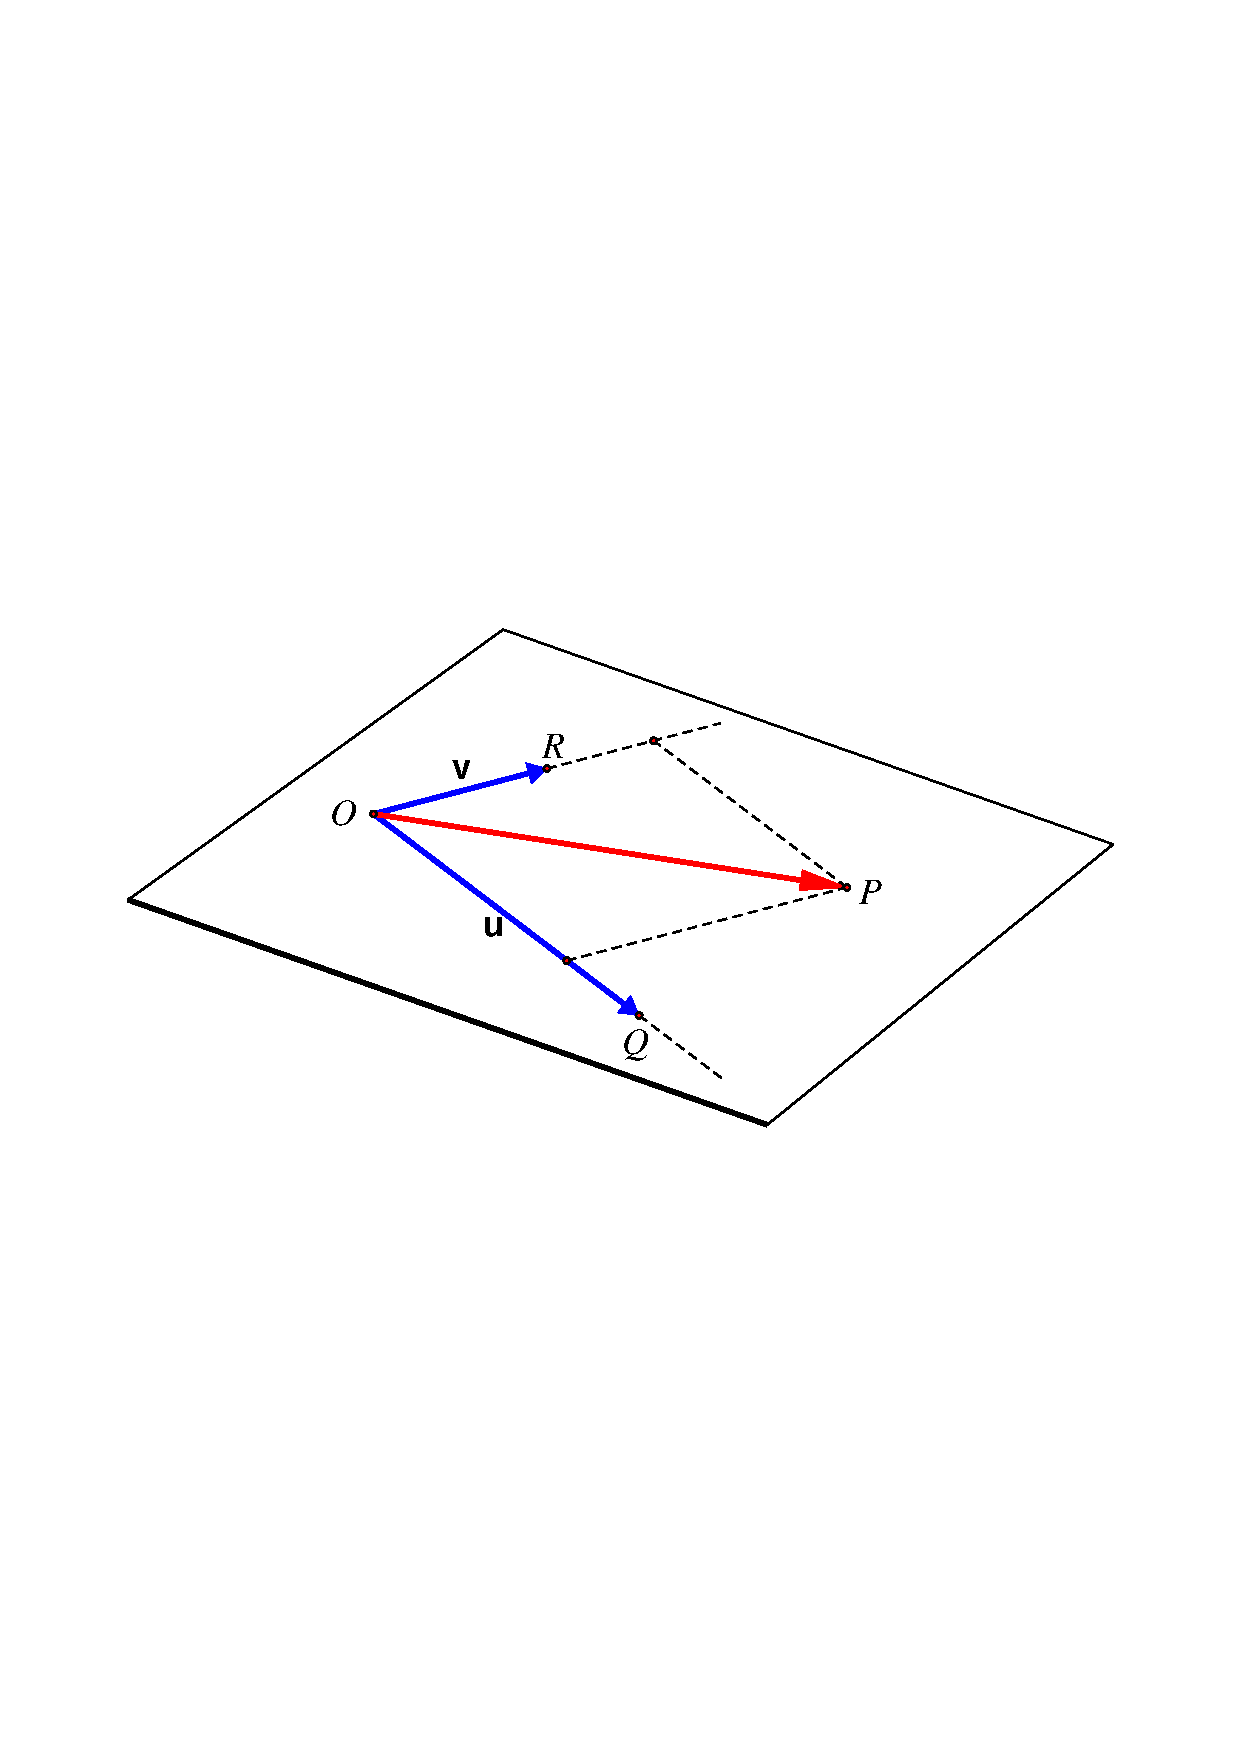
\includegraphics[trim=2cm 10cm 2cm
 10cm,width=0.60\textwidth,clip]{vektor14.pdf}
  \\Figur 7.1: $\mathbf u$ og $\mv$ udspænder en plan i rummet		
\end{center}

\begin{definition}[Udspænding og span]\label{tn7.defSpan}
Ved \ind{udspænding}{udspændingen} af et givet sæt vektorer  ${\mathbf v}_1,\,{\mathbf v}_2,\ldots,{\mathbf v}_p\,$ i et vektorrum $V$ forstås den samlede mængde af alle tænkelige linearkombinationer af vektorerne. Udspændingen af de $p$ vektorer skrives kort
$$
\mathrm{span}\{\mathbf v_1,\mathbf v_2,\ldots,\mathbf v_p\}\,.
$$
\end{definition}

\begin{example}[Linearkombination og span]
Vi betragter i vektorrummet $\mathbb R^{2 \times 3}\,$ de tre matricer/vektorer 
\begin{equation}
\mathbf A=
\begin{matr}{rrr}
 1&0&3\\
 0&2&2\\
 \end{matr}\,,\,\,
\mathbf B=
\begin{matr}{rrr}
 2&1&0\\
 0&3&1\\
 \end{matr}\,\,\mathrm{og}\,\,
\mathbf C=
\begin{matr}{rrr}
 -1&-2&9\\
 0&0&4\\
 \end{matr}\,.
 \end{equation}
 Et eksempel på en linearkombination af de tre vektorer er
 \begin{equation}
 2\mathbf A+0\,\mathbf B +(-1)\mathbf C=
 \begin{matr}{rrr}
 3&2&-3\\
 0&4&0\\
 \end{matr}\,.
 \end{equation}
 Vi har dermed lov til at skrive
 \begin{equation}
  \begin{matr}{rrr}
 3&2&-3\\
 0&4&0\\
 \end{matr}\,\in\, \mathrm{span}\{\mathbf A,\mathbf B,\mathbf C\}\,.
 \end{equation}
 \end{example}
 
\section{Lineær afhængighed og lineær uafhængighed}

To geometriske vektorer $\mathbf u$ og $\mv$ er lineært afhængige, hvis de er parallelle, det vil sige hvis der findes et tal $k$, så $\mv=k\mathbf u$. Mere generelt er et vilkårligt sæt af vektorer lineært afhængige, hvis en af vektorerne er en linearkombination af de øvrige. Dette begreb ønsker vi at overføre til vektorrumsteorien, se den følgende definition.

\begin{definition}[Lineær afhængighed og uafhængighed]\label{defLinafh}
Et sæt bestående af $p$ vektorer $(\mathbf v_1,\mathbf v_2,\ldots,\mathbf v_p)$ i et vektorrum $V$ er \ind{lineær afhængighed}{lineært afhængigt} hvis mindst én af vektorerne kan skrives som en linearkombination af de øvrige, hvis for eksempel
$$
\mv_1=k_2\mv_2+k_3\mv_3+\cdots+k_{p}\mv_{p}\,.
$$
Hvis ingen af vektorerne kan skrives som en linearkombination af de øvrige, kaldes sættet \ind{lineær uafhængighed}{lineært uafhængigt}.\\

NB: Hvis vektorsættet kun består af en enkelt vektor, kaldes sættet lineært afhængigt, hvis det består af 0-vektoren, og ellers lineært uafhængigt.
\end{definition}

\begin{example}[Lineær afhængighed]
Ethvert vektorsæt som indeholder nul-vektoren, er lineært afhængigt! Betragt for eksempel sættet $(\mathbf u,\mv,\mnul,\mathbf w)$, her kan nul-vektoren jo helt trivielt skrives som en linearkombination af de tre andre vektorer i sættet:
$$
\mnul=0\mathbf u+0\mv+0\mathbf w\,,
$$
hvor nul-vektoren er skrevet som en linearkombination af de øvrige vektorer i sættet.
\end{example}

\begin{example}[Lineær afhængighed]
Betragt i vektorrummet $\mathbb R^{2 \times 3}\,$ de tre matricer/vektorer 
\begin{equation}
\mathbf A=
\begin{matr}{rrr}
 1&0&3\\
 0&2&2\\
 \end{matr}\,,\,\,
\mathbf B=
\begin{matr}{rrr}
 2&1&0\\
 0&3&1\\
 \end{matr}\,\,\mathrm{og}\,\,
\mathbf C=
\begin{matr}{rrr}
 -1&-2&9\\
 0&0&4\\
 \end{matr}\,.
 \end{equation}
 $ \mathbf C$ kan skrives som en linearkombination af $ \mathbf A$ og $ \mathbf B$ da der gælder at
 $$
 \mathbf C=3\mathbf A-2\mathbf B\,.
 $$
Derfor er $ \mathbf A$, $ \mathbf B$ og $ \mathbf C$ lineært afhængige.\bs
Derimod er sættet bestående af $\mathbf A$ og $ \mathbf B$ lineært uafhængigt, da de to vektorer ikke er ''parallelle'', idet der tydeligvis ikke findes et tal $k$ således at $ \mathbf B =k \mathbf A$. Ligeså med sættene $(\mathbf A,\mathbf C)$ og $(\mathbf B,\mathbf C)\,$.
\end{example} 

Når man skal undersøge om et sæt af vektorer er lineært afhængigt, så opstår der ved brug definition \ref{defLinafh} spørgsmålet \textit{hvilken} af sættets vektorer der evt. er en linearkombination af de øvrige. Hvor  skal undersøgelsen starte? Dilemmaet kan undgås hvis man i stedet for definitionen bruger den følgende sætning:
 
\begin{theorem}[Lineær afhængighed og uafhængighed]\label{tn7.linafh}
At et vektorsæt  $(\mathbf v_1,\mathbf v_2,\ldots,\mathbf v_p)$ i et vektorrum $V$ er lineært afhængigt, er ensbetydende med at nul-vektoren kan skrives som en egentlig li\-nearkombination af vektorerne. Der skal altså findes skalarer $\,k_1, k_2,\ldots, k_p\,$ som ikke alle er lig med 0, og som opfylder
\begin{equation}
k_1{\mathbf v}_1+k_2{\mathbf v}_2+\cdots+k_p{\mathbf v}_p= \mathbf 0\,.
\end{equation}
I modsat fald er vektorerne lineært uafhængige.
\end{theorem}.

\begin{bevis}
Antag først at $(\mathbf v_1,\mathbf v_2,\ldots,\mathbf v_p)$ er lineært afhængige, så kan én af dem skrives som en linearkombination af de øvrige, for eksempel er
\begin{equation}
\mv_1=k_2\mv_2+k_3\mv_3+\cdots+k_{p}\mv_{p}\,.
\end{equation}
Men dette er ensbetydende med at
\begin{equation}
\mv_1-k_2\mv_2-k_3\mv_3-\cdots-k_{p}\mv_{p}=\mathbf 0\,,
\end{equation}
hvorved nul-vektoren er skrevet som en linearkombination af vektorsættet hvor mindst én af koefficienterne ikke er $0$, da vi jo har koefficienten 1 til $\mv_1$.\bs
Antag omvendt at nul-vektoren er skrevet som en egentlig linearkombination af vektorsættet, hvor for eksempel koefficienten $k_1$ til $\mv_1$ er forskellig fra $0$. Så har vi
\begin{equation}
k_1\mv_1+k_2\mv_2+\cdots+k_{p}\mv_{p}=\mathbf 0\; \Leftrightarrow
\mv_1=(-1)\frac{k_2}{k_1}\mv_2+\cdots+(-1)\frac{k_p}{k_1}\mv_p\,.
\end{equation}
Hermed er $\mv_1$ skrevet som en linearkombination af de øvrige vektorer, og beviset er fuldført.
\end{bevis}

\begin{example}[Lineær afhængighed]
I talrummet $\mathbb R^4$ er der givet vektorerne $\ma=(1,3,0,2)$, $\mb=(-1,9,0,4)$ og $\mc=(2,0,0,1)$. Da der gælder
$$
3\ma-\mb-2\mc=\mathbf 0
$$
er nul-vektoren skrevet som en egentlig linearkombination af de tre vektorer. De er derfor lineært afhængige.
\end{example}

\section{Basis og dimension for et vektorrum}

En afgørende begrundelse for at indføre en basis i et vektorrum er at alle vektorer i vektorrummet derefter kan beskrives ved hjælp af koordinater. I et senere afsnit vi\-ses det hvordan man kan forenkle og standardisere regneopgaver med vektorer når man benytter koordinater. Men i dette afsnit vil vi diskutere de krav, man må stille til en basis og undersøge de teoretiske konsekvenser af kravene.
\bs
En basis for et vektorrum består af et vist antal vektorer opskrevet i en bestemt rækkefølge. En afgørende opgave for basisvektorerne er at udspænde hele vektorrummet, men mere præcist ønsker vi dette job udført af \textit{så få vektorer som muligt}. I så fald viser det sig nemlig at alle vektorer i vektorrummet \textit{på entydig vis} kan skrives som en linearkombination af basisvektorerne. Og det er netop \textit{koefficienterne} i den entydige linearkombination vi vil bruge som koordinater.
\bs
Lad os tage udgangspunkt i nogle karakteristiske egenskaber ved baser for de geo\-metriske vektorer i planen.
\begin{center}
		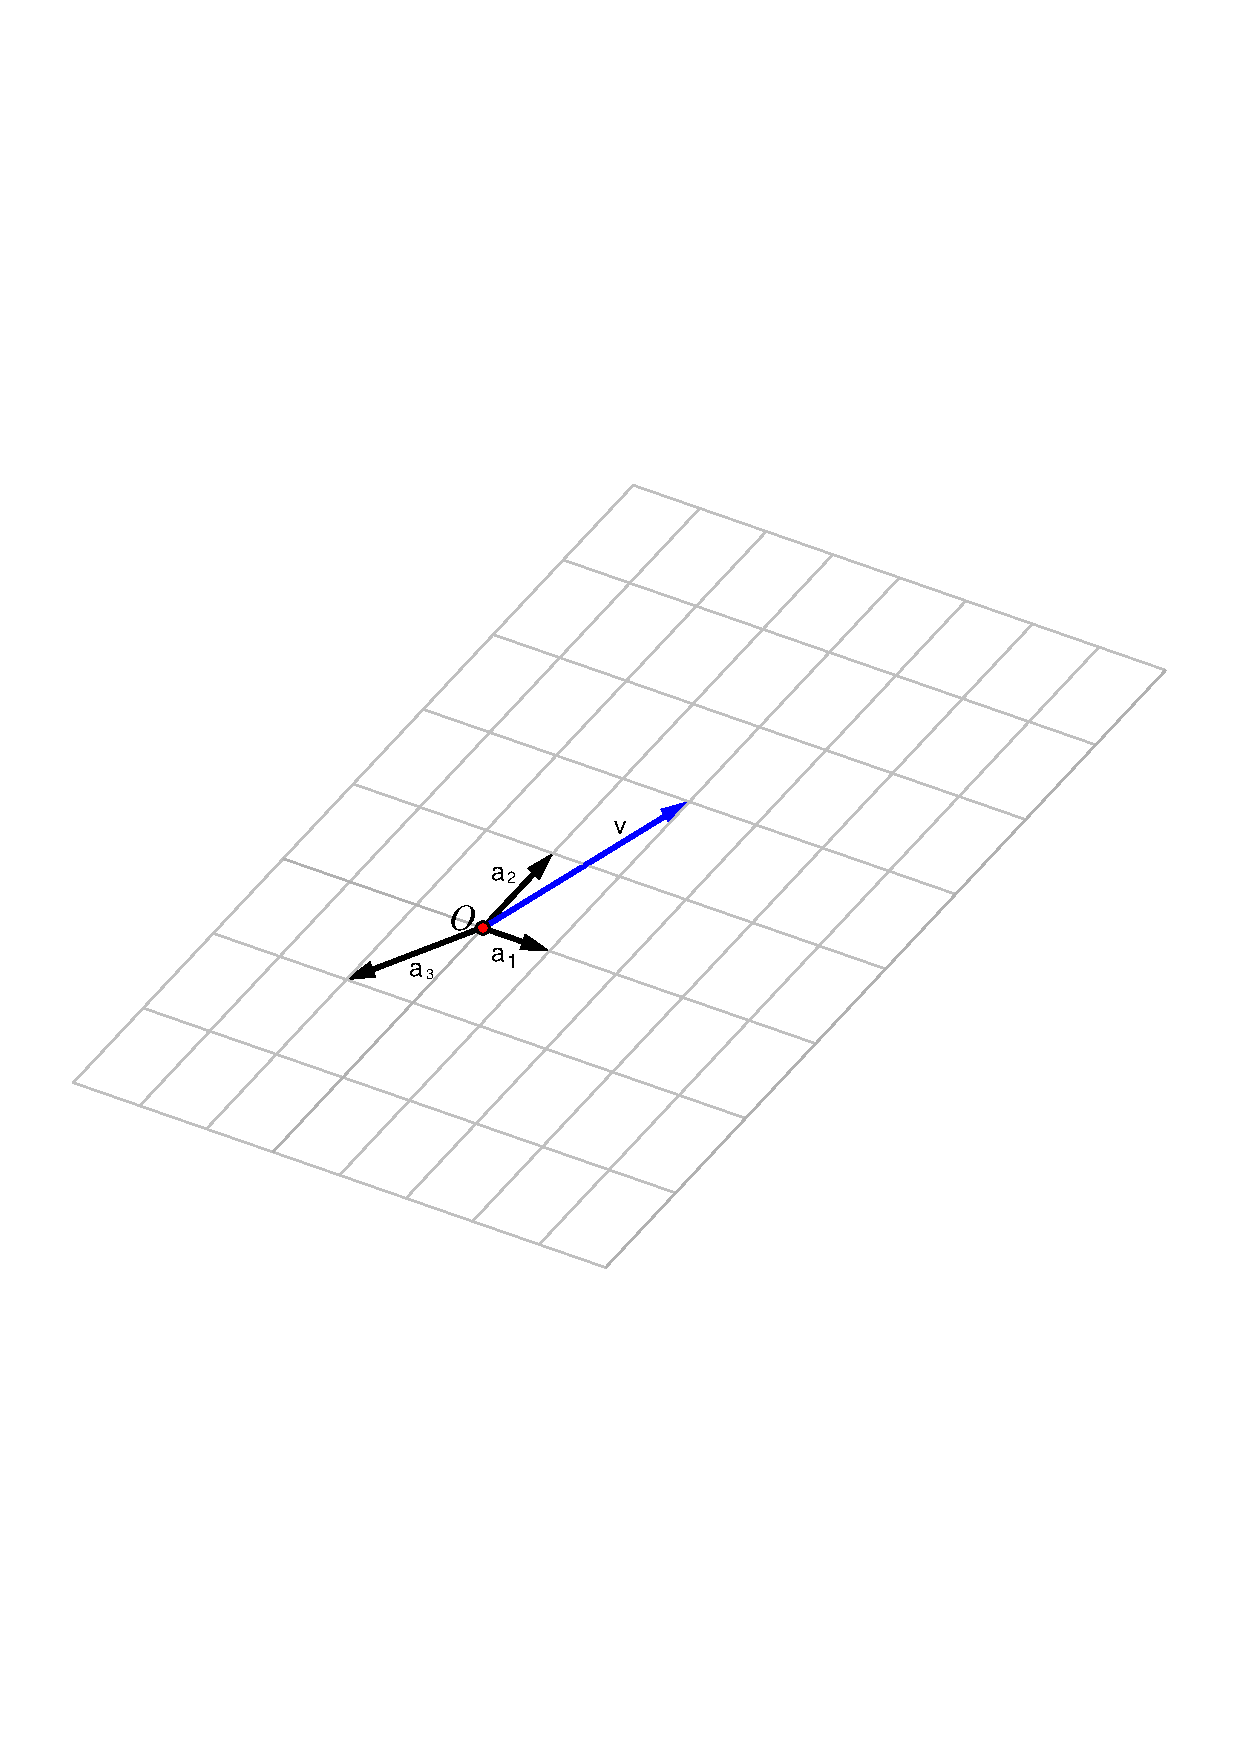
\includegraphics[trim=4cm 12cm 5cm 12cm,width=0.60\textwidth,clip]{linKomb.pdf}	
		\\Figur 7.2: Koordinatsystem i planen med basis $(\ma_1,\ma_2)$			
\end{center}
Betragt vektorsættet $\,(\ma_1,\ma_2,\ma_3)\,$ på figur 7.2, ingen tvivl om at enhver anden vektor i planen kan skrives som en linearkombination af de tre vektorer. Men linearkombinationen er ikke entydig, for eksempel kan vektoren $\mv$ skrives på disse to måder
\begin{align*}
\mv&=2\ma_1+3\ma_2-1\ma_3\\
\mv&=1\ma_1+2\ma_2+0\ma_3\,.
\end{align*}
Problemet er at $a$-vektorerne er lineært afhængige, for eksempel er $\ma_3=-\ma_1-\ma_2\,.$ Men hvis vi fjerner en af dem, for eksempel $\ma_3\,,$ er sættet lineært uafhængigt, og der er så kun én skrivemåde
$$
\mv=1\ma_1+2\ma_2\,.
$$
Vi kan opsummere de karakteristiske egenskaber for en basis for de geometriske vektorer i planen således: (1) enhver basis må bestå af lineært uafhængige vektorer, (2) enhver basis må indeholde netop to vektorer (hvis der er flere end to, er de lineært afhængige, hvis der er færre end to, udspænder de ikke hele vektorrummet), og (3) \textit{ethvert} sæt bestående af to lineært uafhængige vektorer er en basis. Disse egenskaber lader sig overføre til alle andre vektorrum. Det tager vi hul på nu, og vi starter med den generelle definition af en basis.

\begin{definition}[Basis]\label{tn7.defBasis}
Ved en \ind{basis}{basis} for et vektorrum $V$ forstås et ordnet sæt $({\mathbf v}_1,\,{\mathbf v}_2,\ldots,{\mathbf v}_n)\,$ af vektorer fra $V$ som opfylder: 
\begin{enumerate}
\item
$\,({\mathbf v}_1,\,{\mathbf v}_2,\ldots,{\mathbf v}_n)\,$ udspænder $V\,$.
\item
$\,({\mathbf v}_1,\,{\mathbf v}_2,\ldots,{\mathbf v}_n)\,$ er lineært uafhængigt.
\end{enumerate}
\end{definition}

Her bør vi stoppe op og sørge for at definition \ref{tn7.defBasis} faktisk opfylder vores entydighedskrav til en basis. Dette fastslås i den følgende sætning.

\begin{theorem}[Entydighedssætningen]\label{tn7.unik}
Hvis der i et vektorrum $V$ er givet en basis, kan enhver vektor i $V$ skrives som en \textit{unik} linearkombination af basisvektorerne.
\end{theorem}

\begin{bevis}
Vi giver idéen i beviset ved at se på et vektorrum $V$ som har en basis bestående af tre basisvektorer $\,(\ma,\mb,\mc)\,$ og antager at $\mv$ er en vilkårlig vektor i $V$ som på to måder kan skrives som linearkombination af basisvektorerne.  Vi kan da opstille to ligninger
\begin{equation}\label{tn7.basis2}
\begin{array}{c}
\mathbf v=k_1\ma+k_2\mb+k_3\mc\\
\mathbf v=k_4\ma+k_5\mb+k_6\mc
\end{array}
\end{equation}
Ved at trække den nederste ligning i (\ref{tn7.basis2}) fra den øverste opnår vi ligningen
\begin{equation}\label{tn7.basis3}
\mathbf 0=(k_1-k_4)\ma+(k_5-k_2)\mb+(k_3-k_6)\mc\,.
\end{equation}
Da $\ma$, $\mb$ og $\mc$ er lineært uafhængige, kan nul-vektoren kun skrives som en uegentlig linearkombination af dem, derfor er hver af koefficienterne i (\ref{tn7.basis2}) lig med $0$, hvilket medfører at $k_1=k_4$, $k_2=k_5$ og $k_3=k_6$. Men så er de to måder $\mv$ har været skrevet som linearkombination af basisvektorerne på, i virkeligheden den samme, der findes kun én måde! \bs
Dette ræsonnement lader sig umiddelbart udvide til en basis som består af et vilkårligt antal basisvektorer.
\end{bevis}

Vi vender nu tilbage til det faktum at enhver basis for de geometriske vektorer i planen altid indeholder \textit{to} lineært uafhængige basisvektorer, og at der tilsvarende for geometriske vektorer i rummet gælder at en basis må bestå af \textit{tre} lineært uafhængige basisvektorer. Det viser sig at det faste antal basisvektorer er en egenskab ved alle vektorrum der har en basis, og dette gør det muligt at tale om \textit{dimensionen} af et vektorrum som har en basis. For at bevise at egenskaben findes, får vi brug for en hjælpesætning.

\begin{lemma}\label{fundLemma}
Hvis et vektorrum $V$ har en basis bestående af $n$ basisvektorer, så vil ethvert sæt fra $V$ som indeholder mere end $n$ vektorer, være lineært afhængigt.
\end{lemma}

\begin{bevis}
Vi viser idéen i beviset ved at betragte et vektorrum $V$ som har en basis af to vektorer $(\ma,\mb)$, og undersøger tre vilkårlige vektorer $\mc,\mathbf d$ og $\mathbf e$ fra $V$. Vi viser at de tre vektorer nødvendigvis må være lineært afhængige. 
\bs
Da $(\ma,\mb)$ er en basis for $V$, kan vi opstille tre ligninger

\begin{equation}\label{tn7.basis4}
\begin{array}{c}
\mathbf c =c_1\ma+c_2\mb\\
\mathbf d =d_1\ma+d_2\mb\\
\mathbf e =e_1\ma+e_2\mb
\end{array}
\end{equation}

Betragt endvidere nul-vektoren opskrevet ved følgende linearkombination
\begin{equation}\label{tn7.basis5}
x_1\mathbf c+x_2\mathbf d +x_3\mathbf e = \mathbf 0\,,
\end{equation}
der ved indsættelse af ligningerne (\ref{tn7.basis4}) i (\ref{tn7.basis5}) er ensbetydende med

\begin{equation}\label{tn7.basis6}
(x_1c_1+x_2d_1+x_3e_1)\mathbf a +
(x_1c_2+x_2d_2+x_3e_2)\mathbf b =\mathbf 0\,.
\end{equation}
Da nulvektoren kun kan opnås som en linearkombination af $\ma$ og $\mb$, hvis hver af koefficienterne er lig med $0$, er (\ref{tn7.basis6}) ensbetydende med følgende ligningssystem
\begin{equation}\label{tn7.basis7}
\begin{array}{c}
c_1x_1+d_1x_2+e_1x_3=0\\
c_2x_1+d_2x_2+e_2x_3=0
\end{array}
\end{equation}
Dette er et homogent lineært ligningssystem hvor antallet af ligninger er mindre end antallet af ubekendte. Ligningssystemet har derfor uendeligt mange løsninger, hvilket betyder at (\ref{tn7.basis6}) ikke kun er opnåelig under betingelsen af $x_1=0,x_2=0$ og $x_3=0$. Dermed er det vist at sættet $(\mc,\mathbf d,\mathbf e)$ er lineært afhængigt. \bs
Generelt: Antag nu at basen for $V$ består af $n$ vektorer, og at der givet $m$ vektorer fra $V$ hvor $m>n$. Ved at følge samme fremgangsmåde som ovenfor opstår der et homogent lineært ligningssystem bestående af $n$ ligninger med $m$ ubekendte som, fordi $m>n\,$, ligeledes har uendeligt mange løsninger. Derved vises det at de $m$ vektorer er lineært afhængige.
\end{bevis}

Og så er vi klar til at fremsætte den følgende vigtige sætning:

\begin{theorem}[Antal af basisvektorer]\label{tn7.antalBasisvektorer}
Hvis et vektorrum $V$ har en basis bestående af $n$ basisvektorer, så vil enhver basis for $V$ ligeledes bestå af $n$ basisvektorer.
\end{theorem}

\begin{bevis}
Antag at $V$ har to baser med forskelligt antal basisvektorer. Vi kalder basen med færrest basisvektorer for $a$ og den med flest for $b$. I følge \ref{fundLemma} må $b$-basisvektorerne være lineært afhængige, og dette er i modstrid med at de udgør en basis. Antagelsen om at $V$ kan have to baser med forskelligt antal basisvektorer, må derfor være forkert.
\end{bevis}

At antallet af basisvektorer i følge sætning \ref{tn7.antalBasisvektorer} er en \textit{egenskab} ved vektorrum som har en basis, motiverer indførelsen af begrebet dimension:

\begin{definition}[Dimension]\label{tn7.defDim}
Ved dimensionen af et vektorrum $V$ som har en basis b, forstås antallet af basisvektorer i b. Hvis dette antal er $n$, siger man at $V$ er $n$-dimesionalt og skriver
\begin{equation}
\mathrm{dim}(V)=n\,.
\end{equation}
\end{definition}

\begin{example}[Dimension af geometriske vektorrum]
Heldigvis bekræfter definition \ref{tn7.defDim} en intuitiv fornemmelse af at mængden af geometriske vektorer i planen har dimensionen to, og at mængden af geometriske vektorer i rummet har dimensionen tre!
\end{example}

\begin{example}[Standard $e$-basis for talrum]
En vilkårlig vektor $\mv=(a,b,c,d)$ i $\mathbb R^4$ kan på oplagt måde skrives som en linearkombination af fire særlige vektorer i $\mathbb R^4\,:$ 
\begin{equation}\label{tn7.standard1}
\mv=a\,(1,0,0,0)+b\,(0,1,0,0)+c\,(0,0,1,0)+d\,(0,0,0,1)\,.
\end{equation}
Vi sætter 
$\mathbf e_1=(1,0,0,0)$, $\mathbf e_2=(0,1,0,0)$, $\mathbf e_3=(0,0,1,0)$ og $\mathbf e_4=(0,0,0,1)$
og konstaterer ved hjælp af (\ref{tn7.standard1}) at e-sættet $\,(\mathbf e_1,\mathbf e_2,\mathbf e_3,\mathbf e_4)\,$ udspænder $\mathbb R^4$.\bs
 Da det endvidere ses at ingen af vektorerne i e-sættet kan skrives som en linearkombination af de øvrige, er sættet lineært uafhængigt, og $\,(\mathbf e_1,\mathbf e_2,\mathbf e_3,\mathbf e_4)\,$ er dermed en basis for $\mathbb R^4$. Denne særlige basis kaldes \ind{standard e-basis}{standard e-basen} for $\mathbb R^4\,$. Da antallet af basisvektorer i standard e-basen er fire, er dim$(\mathbb R^4)=4\,.$\bs
Dette kan umiddelbart generaliseres til $\mathbb R^n\,$: For ethvert $n$ er e-sættet $\,(\mathbf e_1,\mathbf e_2,\ldots,\mathbf e_n)\,$ hvor 
$$\,\mathbf e_1=(1,0,0,\ldots,0),\,\mathbf e_2=(0,1,0,\ldots,0),\ldots\,,\mathbf e_n=(0,0,0,\ldots,1)$$ en basis for $\mathbb R^n$. Denne særlige basis kaldes \ind{standard e-basis}{standard e-basen} for $\mathbb R^n\,$. Det bemærkes at dim$(\mathbb R^n)=n\,$.
\end{example}

\begin{example}[Standard $e$-basis for matrix-rum]\label{basisForMatricer}
Ved \ind{standard e-basis}{standard e-basen} for vektorrummet $\mathbb R^{2 \times 3}\,$, forstås matrixsættet
\begin{equation}\label{matrixBasis}
\Big(\begin{matr}{rrr}
 1&0&0\\
 0&0&0\\
 \end{matr},
 \begin{matr}{rrr}
 0&1&0\\
 0&0&0\\
 \end{matr},
 \ldots,
 \begin{matr}{rrr}
 0&0&0\\
 0&0&1\\
 \end{matr}\Big)
 \end{equation}
 På samme måde defineres en \textit{standard e-basis} for et vilkårligt matrixrum $\mathbb R^{m \times n}\,$. 
 \end{example}
 \begin{exercise}
 Gør rede for at det matrixsæt, der i eksempel \ref{basisForMatricer} omtales som standard $e$-basis for $\mathbb R^{2 \times 3}\,$, faktisk er en basis for dette vektorrum.
 \end{exercise}

\begin{example}[\textit{Monomiebasen} for polynomiumsrum]
I vektorrummet $P_2(\mathbb R)$ af reelle polynomier af højst 2. grad er vektorsættet $(1,x,x^2)$ en basis. Det ses på følgende måde.
\begin{enumerate}
\item
Ethvert polynomium $P(x)\in P_2(\mathbb R)$ kan skrives på formen
$$P(x)=a_0\cdot 1+a_1\cdot x+a_2\cdot x^2\,,$$
det vil sige som en linearkombination af de tre vektorer i sættet.
\item
Vektorsættet $(1,x,x^2)$ er lineært uafhængigt, idet ligningen
$$
a_0\cdot 1+a_1\cdot x+a_2\cdot x^2=0\;\mathrm{for}\;\;\mathrm{ethvert}\;x
$$
i følge \ind{identitetssætningen for polynomier}{identitetssætningen for polynomier} kun er opfyldt hvis alle koefficienterne $a_0$, $a_1$ og $a_2$ er lig med $0$\,.
\end{enumerate}
Sættet $(1,x,x^2)$ kaldes \ind{monomiebasen}{monomiebasen} eller \ind{standard m-basen}{standard m-basen} for $P_2(\mathbb R)$, og der gælder dim$(P_2(\mathbb R))=3\,$.
\bs
For ethvert $n$ er sættet $(1,x,x^2,\ldots,x^n)$ en basis for $P_n(\mathbb R)$, den kaldes \textit{monomiebasen} eller \textit{standard m-basen} for $P_n(\mathbb R)$. Der gælder derfor dim$(P_n(\mathbb R))=n+1\,$.
\end{example}

I mængden af plane geometriske vektorer kan man vælge et \textit{ethvert} ordnet par af to lineært uafhængige vektorer som  basis. Tilsvarende udgør i rummet \textit{ethvert} sæt af tre lineært uafhængige vektorer en basis. Vi slutter afsnittet af med en videreførsel af dette til generelle n-dimensionale vektorrum:

\begin{theorem}[Tilstrækkelige betingelser for basis]\label{tn7.antalBasisvektorer2}
I et $n$-dimensionalt vektorrum $V$ udgør et vilkårligt ordnet sæt af $n$ lineært uafhængige vektorer fra $V$ en basis for $V\,$.
\end{theorem}
\begin{bevis}
Da $V$ er forudsat $n$-dimensionalt, må det have en basis $b$ bestående af $n$ basisvektorer. Lad $a$-sættet $\,(\ma_1,\ma_2,\cdots,\ma_n)\,$ være et vilkårligt lineært uafhængigt sæt af vektorer fra $V$. Sættet er da en basis for $V$ hvis det udspænder $V$. Antag at dette ikke er tilfældet, og lad $\mv$ være en vektor i $V$ som ikke tilhører span$\{\ma_1,\ma_2,\cdots,\ma_n\}$. Så må   $\,(\mv,\ma_1,\ma_2,\cdots,\ma_n)\,$ være lineært uafhængigt, men dette er i modstrid med sætning \ref{fundLemma} da der er $n+1$ vektorer i sættet. Derfor er antagelsen om at $a$-sættet ikke udspænder $V$ forkert, og det må følgelig være en basis for $V$. 
\end{bevis}

\begin{exercise}
I rummet er der givet to geometriske vektorer $\ma=(1,-2,1)$ og $\mb=(2,-2,0)\,$. Bestem en vektor $\mc$ således at sættet $(\ma,\mb,\mc)$ er en basis for mængden af rumvektorer. 
\end{exercise}

\begin{exercise}
Betragt i det 4-dimensionale vektorrum $\mathbb R^{2\times 2}$ vektorerne
\begin{equation}
\mathbf A=
\begin{matr}{rr}
 1&1\\
 1&0
 \end{matr}\,,\,\,
\mathbf B=
\begin{matr}{rr}
 1&1\\
 0&1
 \end{matr}\,\,\mathrm{og}\,\,
\mathbf C=
\begin{matr}{rr}
 1&0\\
 1&1
 \end{matr}\,.
\end{equation}
Gør rede for at $(\mA,\mB,\mC)$ er et lineært uafhængigt sæt, og supplér sættet op med en 2$\times$2 matrix $\,\mD\,$ således at $\,(\mA,\mB,\mC,\mD)\,$ er en basis for $\,\mathbb R^{2\times 2}\,$.
\end{exercise}

\section{Vektorregning ved hjælp af koordinater}
Koordinater hænger snævert sammen med begrebet basis. Når der i et vektorrum er valgt\- en basis, kan enhver vektor i vektorrummet beskrives ved hjælp af dens koordinater med hensyn til den valgte basis. Vi får hermed et særdeles praktisk alternativ til regneoperationerne addition og multiplikation med skalar, som det oprindeligt er defineret ud fra det  konkrete vektorrums anatomi. I stedet for at udføre de særligt definerede regneoperationerne kan vi blot gennemføre taludregninger med de koordinater der svarer til den valgte basis. Det viser sig endda at vi kan forenkle og standardisere løsningen af typiske opgaver som er fælles for alle vektorrum. Men først giver vi en formel indføring af koordinater med hensyn til en valgt basis.

\begin{definition}[Koordinater mht. given basis]
I et n-dimensionalt vektorrum $V$ er der givet $a$-basen $(\mathbf a_1,\mathbf a_2,\ldots,\ma_n)\,$ samt en vektor $\,\mathbf x$. Vi betragter den unikke linearkombination af basisvektorerne som $\,\mathbf x$ i følge sætning \ref{tn7.unik} kan opskrives ved:
\begin{equation}\label{tn7.koordineter1}
\mathbf x=x_1\mathbf a_1+x_2\mathbf a_2+\cdots +x_n\mathbf a_n\,.
\end{equation}
Koefficienterne $\,x_1,x_2,\ldots,x_n\,$ i (\ref{tn7.koordineter1}) kaldes for $\mathbf x$'s \textit{koordinater med hensyn til basen a}, eller kortere $\mathbf x$'s $a$-koordinater, og de samles i en \textit{a-koordinatvektor} med følgende skrivemåde:
\begin{equation}
_\mathrm a\mathbf x=
\begin{matr}{c}x_1\\x_2\\ \vdots \\x_n \end{matr}\,.
\end{equation}
\end{definition}

\begin{example}[Koordinater mht. en ny basis]
I talrummet $\mathbb R^3$ er der givet en basis \textit{a} ved $\big((0,0,1),(1,2,0),(1,-1,1)\big)$. Endvidere er der givet vektoren $\mv=(7,2,6)$. Da der gælder
$$2\cdot(0,0,1)+3\cdot(1,2,0)+4\cdot(1,-1,1)=(7,2,6)\,$$
ser vi at
$$
_\mathrm a\mathbf v=\begin{matr}{r}2\\3\\4 \end{matr}\,.
$$
Vektoren $(7,2,6)$ har dermed $a$-koordinaterne $(2,3,4)\,$.
\end{example}

For at kunne jonglere med mange vektorers koordinater i diverse regneopgaver får vi brug for følgende vigtige sætning.

\begin{theorem}[Koordinatsætningen]\label{tn7.koord_linearitet}
I et vektorrum $V$ er der givet to vektorer $\mathbf u$ og $\mathbf v$ samt et reelt tal $\,k\,$. Der er endvidere valgt en vilkårlig basis $a$. De to regneoperationer $\mathbf u + \mathbf v$ og $k\,\mathbf u$ kan da udføres ved hjælp af $a$-koordinaterne således:
\begin{enumerate}
\item
$_\mathrm a(\mathbf u+\mathbf v)={_\mathrm{a}\mathbf{u}}+{_\mathrm a\mathbf v}$
\item
$_\mathrm a(k\mathbf u)=k\,_\mathrm a\mathbf u$
\end{enumerate}

Sagt med ord: Koordinaterne for en vektorsum fås ved at lægge koordinaterne for vektorerne sammen, og koordinaterne for en vektor ganget med et tal er vektorens koordinater ganget med tallet. 
\end{theorem}\label{tn6.koordinater}
\begin{proof}
Se beviset for den tilsvarende sætning for geometriske vektorer i rummet, \tref{NUID12-tn6.koord_linearitet}{sætning}. Beviset for det generelle tilfælde fås som en simpel udvidelse.
\end{proof}
\begin{example}[Vektorregning ved hjælp af koordinater]
Vi udfører nu en vektorregning ved hjælp af koordinater. Eksemplet er ikke specielt mate\-matisk interessant, men vi gennemfører det detaljeret for at demonstrere teknikken i sætning \ref{tn7.koord_linearitet}.\bs
Der er givet tre polynomier i vektorrummet $P_2(\mathbb R)$: $$R(x)=2-3x-x^2\,,S(x)=1-x+3x^2\,\,\,\mathrm{og}\,\,\, T(x)=x+2x^2\,.$$
Opgaven går ud på at bestemme polynomiet $P(x)=2R(x)-S(x)+3T(x)\,$. Vi vælger at udføre den ved hjælp af koordinaterne for polynomierne med hensyn til \ind{standard m-basis}{standard m-basis} for $P_2(\mathbb R)$.
\begin{align*}
_\mathrm mP(x) &=\,{_\mathrm m\big(2R(x)-S(x)+3T(x)\big)}
\smallskip\\
&=\,{_\mathrm m(2R(x))}+{_\mathrm m(-S(x))}+{_\mathrm m(3T(x))}
\smallskip\\
&=\,2\,{_\mathrm mR(x)}-{_\mathrm mS(x)}+3\,{_\mathrm mT(x)}
\smallskip\\
&=\,2\begin{matr}{r}2\\-3\\-1\end{matr}-\begin{matr}{r}1\\-1\\3\end{matr}+3\begin{matr}{r}0\\1\\2\end{matr}=\begin{matr}{r}3\\-2\\1\end{matr}\,.
\end{align*}
Nu oversætter vi tilbage fra den fundne koordinatvektor til det ønskede polynomium: $$\,P(x)=3-2x+x^2\,.$$
\end{example}

\section{Om brug af koordinatmatricer}\label{tn7.AfsnitKoordMatrix}
Når man giver sig i kast med opgaver om vektorer og benytter sig af deres koordinater med hensyn til en given basis, fører det meget ofte til at man opstiller et lineært ligningssystem og løser opgaven ved hjælp af matrixregning. En matrix påkalder sig særlig opmærksomhed, nemlig den der fremkommer når man sætter nogle vektorers koordinatsøjler sammen til en \textit{koordinatmatrix}:
\begin{explain}[Koordinatmatrix for vektorsæt]
Hvis der i et $n$-dimensionalt vektorrum $V$ findes en basis $a$, og der er givet et ordnet sæt af $m$ vektorer, opstår sættets \ind{koordinatmatrix}{a-koordinatmatrix} ved at man i den givne rækkefølge stiller vektorernes $a$-koordinatsøjler sammen til en \textit{m}$\times$\textit{n} matrix.
\medskip\\
Tag for eksempel et sæt bestående af tre vektorer i $\mathbb R^2:$  $\,\big((1,2),(3,4),(5,6)\big )\,$. Sættets koordinatmatrix med hensyn til standard $e$-basen for  $\mathbb R^2\,$ er 2$\times$3-matricen
$$
\begin{matr}{rrr}1&3&5\\2&4&6 \end{matr}\,.
$$
\end{explain}

Vi vil nu vise hvordan koordinatmatricer opstår igennem en række eksempler som vi for afvekslingens skyld tager fra forskellige vektorrum. Metoderne lader sig umiddelbart bruge på andre vektorrumstyper, og efter hvert eksempel gengiver vi metoden i en koncentreret og generel form.

\begin{obs}
Det er vigtigt for din samlede forståelse af vektorrumsteorien at du selv øver dig i og indser hvordan koordinatmatricer faktisk opstår når man er i gang med typiske opgaver.
\end{obs}
\subsection{Om en vektor er linearkombination af andre vektorer}
Der er i $\mathbb R^4$ givet fire vektorer
\begin{align*}
\mathbf a_1 &= (1,1,1,1)\\
\mathbf a_2 &= (1,0,0,1)\\
\mathbf a_3 &= (2,3,1,4)\\
\mathbf b &= (2,-2,0,1)
\end{align*}
\textit{Opgave}: Undersøg om $\mb$ er en linearkombination af $\mathbf a_1$, $\mathbf a_2$ og $\mathbf a_3$\,.
\medskip\\
\textit{Løsning}: Vi skal undersøge om der findes $\,x_1,\,x_2,\,x_3\in\mathbb R\,$ således at
\begin{equation}\label{tn7.linkombEx}
x_1\ma_1+x_2\ma_2+x_3\ma_3=\mb\,.
\end{equation}
Ved hjælp af sætning \ref{tn7.koord_linearitet} kan vi omskrive (\ref{tn7.linkombEx}) til e-koordinatvektorligningen
$$
x_1\begin{matr}{r}1\\1\\1\\1\end{matr}+
x_2\begin{matr}{r}1\\0\\0\\1\end{matr}+
x_3\begin{matr}{r}2\\3\\1\\4\end{matr}=
\begin{matr}{r}2\\-2\\0\\1\end{matr}
$$
som er ensbetydende med det lineære ligningssystem
\begin{align*}
x_1+x_2+2x_3&=2\\
x_1+3x_3&=-2\\
x_1+x_3&=0\\
x_1+x_2+4x_3&=1
\end{align*}
Vi opstiller ligningssystemets totalmatrix og angiver (uden mellemregninger) dens trappeform
\begin{equation}\label{tn7.linkombEx2}
\mathbf T=
\begin{matr}{rrrr}1&1&2&2\\1&0&3&-2\\1&0&1&0\\1&1&4&1\end{matr}
\;\Rightarrow \;
\mathrm{trap}(\mathbf T)=\begin{matr}{rrrr}1&0&0&0\\0&1&0&0\\0&0&1&0\\0&0&0&1\end{matr}\,.
\end{equation}
Af (\ref{tn7.linkombEx2}) ses det at rangen af ligningssystemets kofficientmatrix er 3, mens rangen af totalmatricen er 4. Ligningssystemet har derfor ingen løsninger. Dette medfører at (\ref{tn7.linkombEx}) ikke kan løses. Vi konkluderer 
$$\mb \notin \mathrm{span}\{\ma_1,\ma_2,\ma_3\}\,.$$

\begin{method}[Linearkombination]\label{tn7.methLinKomb}
Man kan afgøre om en given vektor $\mb$ er en linarkombination af andre vektorer $\,\ma_1,\,\ma_2,\ldots,\ma_p\,$ ved at løse det lineære ligningssystem hvis totalmatrix er identisk med koordinatmatricen for $\,(\ma_1,\ma_2,\ldots,\ma_p,\mb\,)$ med hensyn til en given basis.\bs
NB: Generelt kan der være ingen, eller én eller uendeligt mange måder hvorpå vektoren kan skrives som linearkombinationer af de øvrige.
\end{method}

\subsection{Om vektorer er lineært afhængige} \label{tn7.seclinaf}
Vi betragter i vektorrummet $\mathbb R^{2 \times 3}\,$ de tre matricer: 
\begin{equation}
\mathbf A=
\begin{matr}{rrr}
 1&0&3\\
 0&2&2
 \end{matr}\,,\,\,
\mathbf B=
\begin{matr}{rrr}
 2&1&0\\
 0&3&1
 \end{matr}\,\,\mathrm{og}\,\,
\mathbf C=
\begin{matr}{rrr}
 -1&-2&9\\
 0&0&4
 \end{matr}\,.
 \end{equation}
\textit{Opgave}: Undersøg om de tre matricer er lineært afhængige.\bs
 \textit{Løsning}: Vi benytter sætning \ref{tn7.linafh} og forsøger at finde tre reelle tal $\,x_1\,$, $\,x_2\,$ og $\,x_3\,$ som ikke alle er lig med $0$, men som opfylder 
 \begin{equation}\label{tn7.linafhEx}
 x_1\mathbf A+x_2\mathbf B+x_3\mathbf C
 =\begin{matr}{rrr}
 0&0&0\\
 0&0&0
 \end{matr}\,.
 \end{equation}
 Ved hjælp af sætning \ref{tn7.koord_linearitet} kan vi omskrive (\ref{tn7.linafhEx}) til e-koordinatvektorligningen
$$
x_1\begin{matr}{r}1\\0\\3\\0\\2\\2\end{matr}+
x_2\begin{matr}{r}2\\1\\0\\0\\3\\1\end{matr}+
x_3\begin{matr}{r}-1\\-2\\9\\0\\0\\4\end{matr}=
\begin{matr}{r}0\\0\\0\\0\\0\\0\end{matr}
$$
som er ensbetydende med det homogene lineære ligningssystem hvis totalmatrix her opstilles sammen med dens trappeform (mellemregninger udelades):
\begin{equation}\label{tn7.linafhEx2}
\mathbf T=
\begin{matr}{rrrr}1&2&-1&0\\0&1&-2&0\\3&0&9&0\\0&0&0&0\\2&3&0&0\\2&1&4&0
\end{matr}
\;\Rightarrow \;
\mathrm{trap}(\mathbf T)=\begin{matr}{rrrr}
1&0&3&0\\0&1&-2&0\\0&0&0&0\\0&0&0&0\\0&0&0&0\\0&0&0&0
\end{matr}\,.
\end{equation}
Af (\ref{tn7.linafhEx2}) ses at såvel ligningssystems koefficientmatrix som dets totalmatrix har rangen 2, og da antallet af ubekendte er større, nemlig 3, konkluderer vi at ligningen (\ref{tn7.linafhEx}) har uendeligt mange løsninger, se \tref{NUID1-TN2.11c2}{sætning}. Derfor er de tre matricer lineært afhængige, for eksempel kan man af $\,\mathrm{trap}(\mathbf T)$ udlede at  
$$-3\mathbf A+2\mathbf B+\mathbf C=\begin{matr}{rrr}
 0&0&0\\
 0&0&0
 \end{matr}\,.$$

\begin{method}[Lineær afhængighed eller uafhængighed]\label{tn7.methLinAfh}
Man kan afgøre om vektorerne $\,\mv_1,\,\mv_2,\ldots,\mv_p\,$ er lineært afhængige ved at løse det homogene lineære ligningssystem hvis totalmatrix er identisk med koordinatmatricen for $\,(\mv_1,\mv_2,\ldots,\mv_p,\mnul)$ med hensyn til en given basis.\bs
NB: Da ligningssystemet er homogent, er der én løsning eller uendeligt mange løsninger. Hvis rangen af koordinatmatricen er lig med $p$, er der  én løsning, denne løsning må være nul-løsningen, og de $p$ vektorer er derfor lineært uafhængige. Hvis rangen af koordinatmatricen er mindre end $p$, er der uendeligt mange løsninger. Der findes altså andre løsninger end nulløsningen, og de $p$ vektorer er derfor lineært afhængige.
\end{method} 

\subsection{Om et sæt af vektorer er en basis} \label{tn7.secvekbas}

I et $n$-dimensionalt vektorrum kræves der $n$ basisvektorer, se sætning \ref{tn7.antalBasisvektorer}. Når man bliver spurgt om et forelagt sæt af vektorer kan være en basis, kan man straks slutte at dette ikke er tilfældet hvis antallet af vektorer i sættet er mindre end eller større end $n$. Men hvis der \textit{er} $n$ vektorer i sættet, behøver man ifølge sætning \ref{tn7.antalBasisvektorer2} kun undersøge om sættet er lineært uafhængigt, og her har vi allerede metode \ref{tn7.methLinAfh} at gå frem efter. Vi kan dog på en interessant måde videreudvikle metoden, idet vi kan bringe determinanten af vektorsættets koordinatmatrix i spil!
\medskip\\
Lad os for eksempel undersøge om polynomierne 
$$P_1(x)=1+2x^2,\,P_2(x)=2-x+x^2\;\;\mathrm{og}\;\; P_3(x)=2x+x^2$$
udgør en basis for $P_2(\mathbb R)$. Da dim$(P_2(\mathbb R))$ = 3, er antallet af polynomier i orden. For at undersøge om de også er lineært uafhængige, benytter vi deres koordinatvektorer med hensyn til \ind{monomiebasis}{monomiebasen} og opstiller ligningen
$$
x_1\begin{matr}{r}1\\0\\2\end{matr}+
x_2\begin{matr}{r}2\\-1\\1\end{matr}+
x_3\begin{matr}{r}0\\2\\1\end{matr}=
\begin{matr}{r}0\\0\\0\end{matr}\,
$$
som, hvis der er lineært uafhængigt,  kun må løsningen $\,x_1=x_2=x_3=0\,$. Ligningen er ensbetydende med et homogent lineært ligningssystem bestående af 3 ligninger med 3 ubekendte. Systemets koefficientmatrix og totalmatrix er:
$$
\mathbf A=
\begin{matr}{rrr}1&2&0\\0&-1&2\\2&1&1\end{matr}
\;\;\mathrm{og}\;\;
\mathbf T=
\begin{matr}{rrr|r}1&2&0&0\\0&-1&2&0\\2&1&1&0\end{matr}\,.
$$
Som for ethvert homogent lineært ligningssystem består totalmatricens højreside af lutter $0$'er, derfor er det på forhånd givet at $\rho(\mathbf A)=\rho(\mathbf T)$, og at der \textit{er} løsninger. Der er én løsning netop når $\rho(\mathbf A)$ er lig med antallet af ubekendte, det vil sige 3. Og denne løsning må da være nul-løsningen $\,x_1=x_2=x_3=0\,$ idet $L_{hom}\,$ altid indeholder nul-løsningen. \bs
Her kan vi udnytte at $\mathbf A$ er en kvadratisk matrix og dermed har en \textit{determinant}. $\mathbf A$ har fuld rang, netop når den er \textit{regulær}, det vil sige $\mathrm{det}(\mathbf A)\neq0$.\bs
Da udregning viser at $\mathrm{det}(\mathbf A)=5\,$ kan vi konkludere at $\,\big(P_1(x),P_2(x),P_3(x)\big)\,$ udgør en basis for $P_2(\mathbb R)\,$.

\begin{method}[Bevis for basis]\label{tn7.methBasis}
Når man i et $n$-dimensionalt vektorrum $V$ skal afgøre om et vektorsæt bestående af $n$ vektorer $(\mv_1,\mv_2,\ldots,\mv_n)$ er en basis for $V$, behøver man blot undersøge om sættet er lineært uafhængigt. En særlig mulighed for at undersøge dette opstår ved at vektorsættets koordinatmatrix er en kvadratisk \textit{n}$\times$\textit{n} matrix:
\medskip\\
Sættet udgør en basis for $V$ netop når determinanten af sættets koordinatmatrix med hensyn til en basis $a$ er forskellig fra $0$, kort sagt
\begin{equation}
(\mv_1,\mv_2,\ldots,\mv_n)\,\,\mathrm{er}\,\,\mathrm{en}\,\,\mathrm{basis}
\,\,
\Leftrightarrow\,\,
\mathrm{det}\!\left(\begin{matr}{cccc} \vekind av_1 & \vekind av_2 & \cdots & \vekind av_n \end{matr} \right)\neq 0\,.
\end{equation}
\end{method}

\subsection{At finde de nye koordinater når der skiftes basis} \label{tn7.secbasisskifte}

Et teknisk problem af afgørende betydning for videregående brug af lineær algebra, er at kunne udregne nye koordinater for en vektor når der vælges ny basis. I den sammenhæng får en særlig \textit{basisskiftematrix} en vigtig rolle. Vi demonstrerer nu hvordan basismatricer opstår.\bs
I et 3-dimensionalt vektorrum $V$ er der givet en basis $a$. Der vælges nu en ny basis $b$ som er bestemt ved basisvektorernes $a$-koordinater:
$$
\vekind ab_1=\begin{matr}{r}1\\1\\1\end{matr}\,,\;
\vekind ab_2=\begin{matr}{r}1\\0\\2\end{matr}\,\;\mathrm{og}\,\;
\vekind ab_3=\begin{matr}{r}2\\3\\0\end{matr}\,.
$$
\textit{Opgave 1}: Bestem $a$-koordinaterne for en vektor $\mv$ som er givet ved $b$-koordinater således:
\begin{equation}\label{tn7.bkoordGivet}
\vekind bv=\begin{matr}{r}5\\-4\\-1\end{matr}\,.
\end{equation}

\textit{Løsning}:
Udtrykket (\ref{tn7.bkoordGivet}) svarer til vektorligningen
$$
\mv=5\mb_1-4\mb_2-1\mb_3\
$$
som vi nedenfor først omsætter til en $a$-koordinatvektorligning, hvis højreside vi vælger at omskrive til et matrix-vektorprodukt, før vi til sidst udregner facit: 
\begin{align*}
\vekind av&= 5\,\begin{matr}{r}1\\1\\1\end{matr}-4\,\begin{matr}{r}1\\0\\2\end{matr}-1\begin{matr}{r}2\\3\\0\end{matr}
\medskip\\
&=\begin{matr}{rrr}1&1&2\\1&0&3\\1&2&0\end{matr}\,
\begin{matr}{r}5\\-4\\-1\end{matr}=
\begin{matr}{r}-1\\2\\-3\end{matr}\,.
\end{align*}
Bemærk at 3$\times$3-matricen i den sidste ligning er koordinatmatricen for $b$-basisvektorerne med hensyn til $a$-basen. Den spiller en vigtig rolle, da vi åbenbart kan finde $a$-koordinaterne for $\mv$ ved at gange den med $b$-koordinatervektoren for $\mv$! Matricen får derfor betegnelsen \textit{basisskiftematrix}, dens egenskab er at den oversætter $b$-koordinater til $a$-koordinater, og den tildeles symbolet $\,\matind aMb\,$. Koordinatskifterelationen kan da skrives på denne bekvemme måde
\begin{equation}\label{tn7.basisskifte}
\vekind av = \matind aMb\,\vekind bv\,.
\end{equation}

\textit{Opgave 2}: Bestem $b$-koordinaterne for en vektor $\mathbf u$ som er givet ved $a$-koordinaterne således:
\begin{equation}\label{tn7.akoordGivet}
\vekind au=\begin{matr}{r}1\\2\\3\end{matr}\,.
\end{equation}

\textit{Løsning}: Da $\matind aMb$ er koordinatmatrix for en basis er den \textit{regulær} og har dermed en invers matrix. Vi kan derfor benytte koordinatskifterelationen (\ref{tn7.basisskifte}) således:
\begin{align*}
\vekind au &= \matind aMb\,\vekind bu\,\Leftrightarrow\\
{\matind aMb}^{-1}\,\vekind au &= {\matind aMb}^{-1}\,\matind aMb\,\vekind bu\,\Leftrightarrow\\
\vekind bu &= {\matind aMb}^{-1}\,\vekind au\,\Leftrightarrow\\
\vekind bu&={\begin{matr}{rrr}1&1&2\\1&0&3\\1&2&0\end{matr}}^{-1}\,\begin{matr}{r}1\\2\\3\end{matr}=\begin{matr}{r}11\\-4\\-3\end{matr}\,.
\end{align*}

\begin{method}[Koordinatskifte ved basisskifte]\label{tn7.methSkifte}
Når der i et vektorrum er der givet en basis $a\,$, og når en ny basis $b$ kendes ud fra dens basisvektorers $a$-koordinater, opstilles \ind{basisskiftematrix}{basisskiftematricen} $\matind aMb$ som er identisk med $a$-koordinatmatricen for $b$-basisvektorerne.
\begin{enumerate}
\item
Hvis $b$-koordinaterne for en vektor $\mv$ er kendte, kan dens $a$-koordinater findes ved matrix-vektorproduktet:
$$
\vekind av = \matind aMb\,\vekind bv\,.
$$
\item
Hvis det omvendt er $a$-koordinaterne for $\mv$ som er kendte, kan dens $b$-koordinater findes ved matrix-vektorproduktet:
$$
\vekind bv = {\matind aMb}^{-1}\,\vekind av\,.
$$
Kort sagt er den basisskiftematrix der oversætter  $a$-koordinater til $b$-koordinater, den inverse til den basisskiftematrix der oversætter $b$-koordinater til $a$-koordinater:
$$ \matind bMa=(\matind aMb)^{-1}\,.$$
\end{enumerate}
\end{method}

\section{Underrum}

Ofte kommer man ud for at en delmængde af et vektorrum i sig selv er et vektorrum. På figur 7.3 ses to stedvektorer $\stackrel{\rightarrow}{OP}$ og $\stackrel{\rightarrow}{OQ}$ som udspænder planen $F\,$: 

\begin{center}
		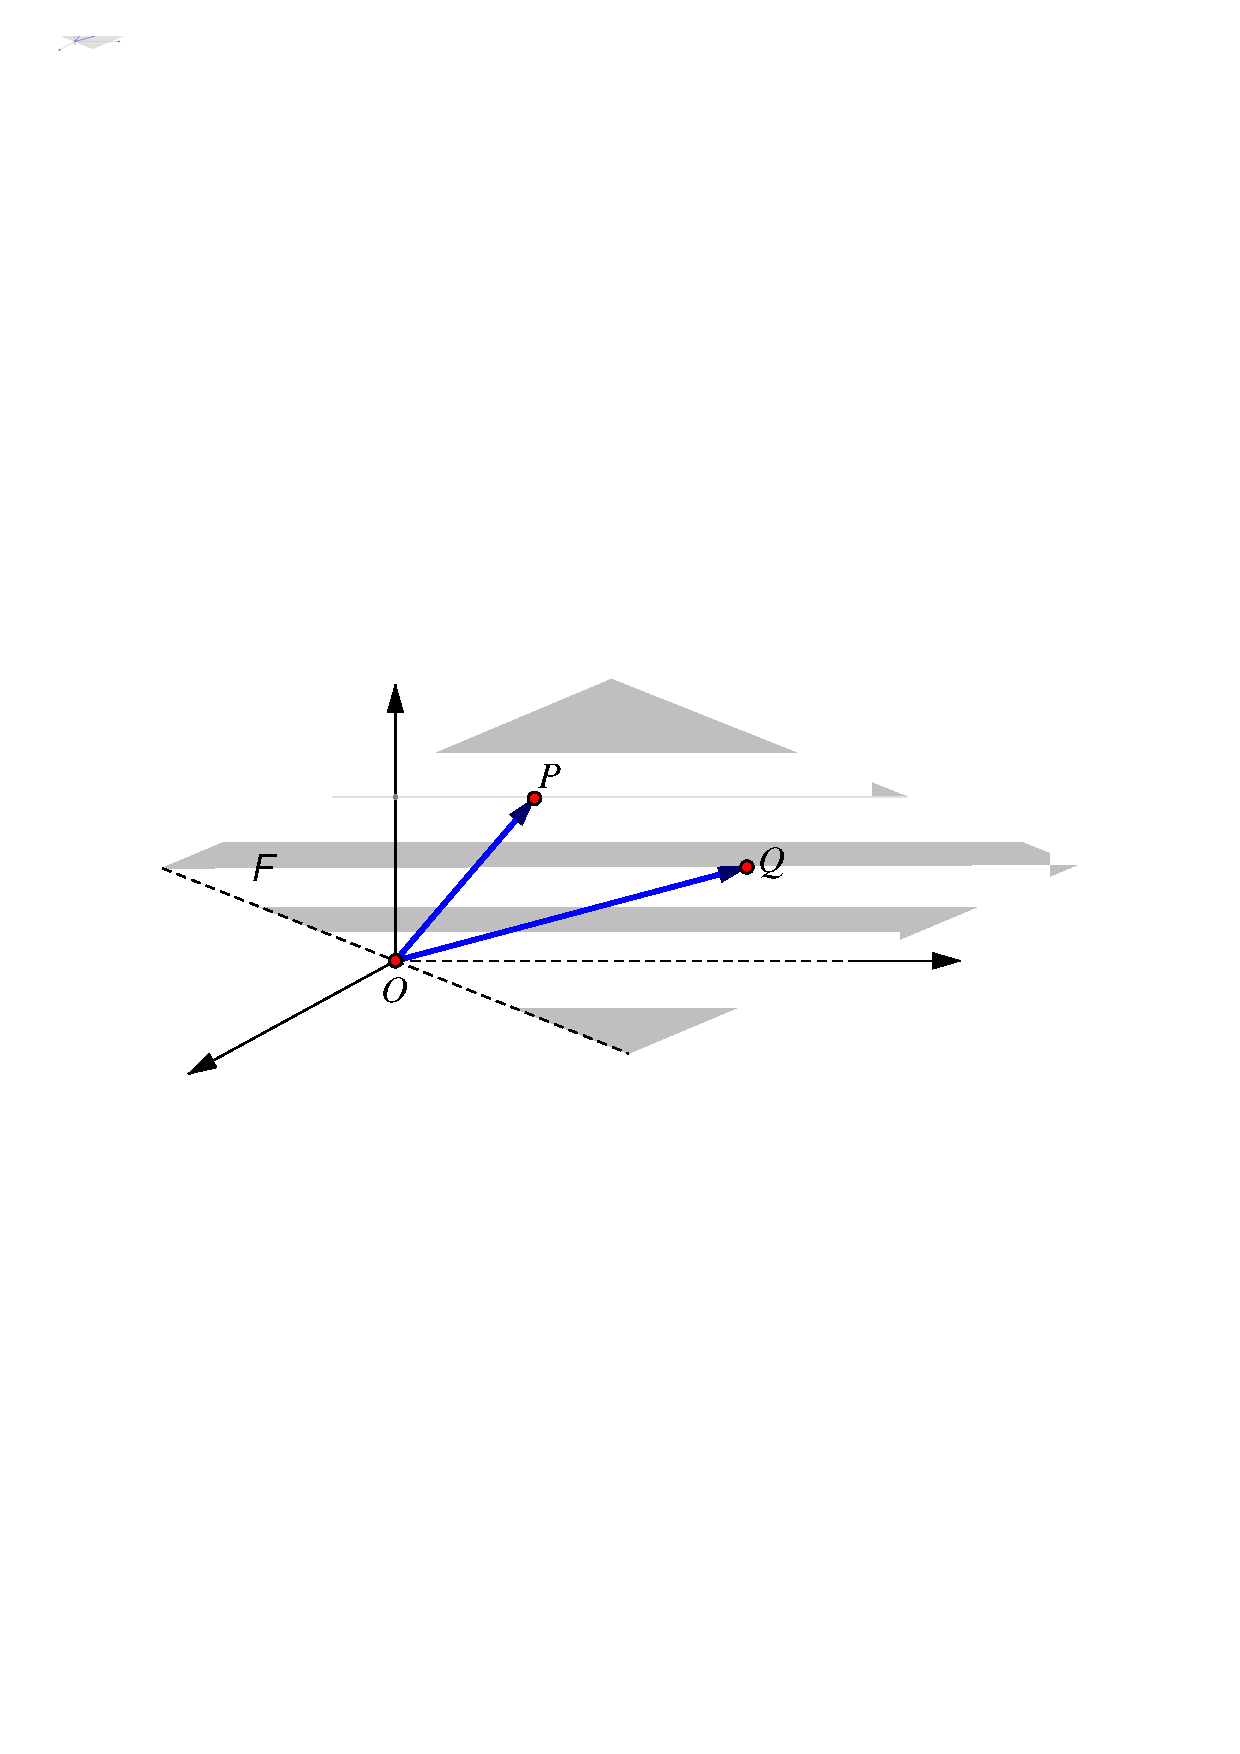
\includegraphics[trim=2cm 10cm 2cm
 10cm,width=0.60\textwidth,clip]{span.pdf}
  \\Figur 7.3: En plan gennem origo fortolket som et \textit{underrum} i rummet		
\end{center}
Da span$\{\stackrel{\rightarrow}{OP},\stackrel{\rightarrow}{OQ}\}$ kan betragtes som et selvstændigt (2-dimensionalt) vektorrum, omtales det som et \textit{underrum} i det (3-dimensionale) vektorrum af stedvektorer i rummet.

\begin{definition}[Underrum]\label{tn7.defUrum}
En delmængde $U$ af et vektorum $V$ kaldes et \ind{underrum}{underrum} i $V$ hvis det i sig selv er et vektorrum.
\end{definition}
\begin{aha}
I ethvert vektorrum V kan man straks udpege to underrum:\\
$1)\,\,$ V er selv et underrum i V.\\
$2)\,\,$ Mængden $\,\left\{\,\mnul\,\right\}\,$ er et underrum i V.\\
Disse underrum kaldes de \textit{trivielle} underrum i V. 
\end{aha}
Når man skal tjekke om en delmængde er et underrum, behøver man kun at undersøge om stabilitetskravene er opfyldte. Dette fremgår af følgende sætning.

\begin{theorem}[Tilstrækkelige betingelser for underrum] \label{tn7.stabilNok}
En delmængde $U$ af et vektorum $V$ er et underrum i $V$ hvis $U$ er \textit{stabil} med hensyn til addition og multiplikation med skalar. Det betyder
\begin{enumerate}
\item
Summen af to vektorer fra $U$ tilhører også $U\,$.
\item
Produktet af en vektor i $U$ med en skalar tilhører også $U\,$.
\end{enumerate}
\end{theorem}
\begin{bevis}
Da $U$ opfylder de to stabilitetskrav i definition \ref{tn7.defVektorrum}, mangler vi blot at argumentere for at $U$ også overholder de otte regneregler i definitionen. Men dette er klart, da alle vektorer i $U$ også er vektorer i $V$ hvor de gælder.
\end{bevis}
\begin{example}[Basis for et underrum]
Vi betragter en delmængde $M_1$ af $\,\mathbb R^{2\times 2}\,$, som består af alle matricer af typen
\begin{equation}\label{tn7.matrixSubset}
\begin{matr}{rr}a&b\\b&a\end{matr}
\end{equation}
hvor $a$ og $b$ er vilkårlige reelle tal. Vi prøver at lægge to matricer af typen (\ref{tn7.matrixSubset}) sammen
$$
\begin{matr}{rr}1&2\\2&1\end{matr}+\begin{matr}{rr}3&4\\4&3\end{matr}=\begin{matr}{rr}4&6\\6&4\end{matr}
$$
og vi ganger en af typen (\ref{tn7.matrixSubset}) med en skalar
$$ 
-3\,\begin{matr}{rr}2&-3\\-3&2\end{matr}=\begin{matr}{rr}-6&9\\9&-6\end{matr}\,.
$$
I begge tilfælde er den resulterende matrix af typen (\ref{tn7.matrixSubset}), og det er klart at det samme ville være tilfældet hvis vi havde brugt andre. $M_1$ opfylder derfor stabilitetskravene for et vektorrum. Det følger derfor af sætning \ref{tn7.stabilNok} at $M_1$ er et underrum i $\,\mathbb R^{2\times 2}\,$. \bs
Bemærk endvidere at $M_1$ udspændes af to lineært uafhængige 2$\times$2 matricer idet
$$
\begin{matr}{rr}a&b\\b&a\end{matr}=a\,\begin{matr}{rr}1&0\\0&1\end{matr}+b\,\begin{matr}{rr}0&1\\1&0\end{matr}\,.
$$
Derfor er $M_1$ et 2-dimensionalt underrum i $\,\mathbb R^{2\times 2}\,$, og en mulig basis for $M_1$ er givet ved
$$\Big (\begin{matr}{rr}1&0\\0&1\end{matr},\begin{matr}{rr}0&1\\1&0\end{matr}\Big )\,.
$$ 
\end{example}

\begin{example}[Delmængde som ikke er et underrum]
Delmængden $M_2$ af $\,\mathbb R^{2\times 2}\,$ består af alle matricer af typen
\begin{equation}\label{tn7.matrixSubset2}
\begin{matr}{cr}a&b\\a\cdot b&0\end{matr}\,
\end{equation}
hvor $a$ og $b$ er vilkårlige reelle tal. Vi prøver at lægge to matricer af typen (\ref{tn7.matrixSubset2}) sammen
$$
\begin{matr}{rr}1&2\\2&0\end{matr}+\begin{matr}{rr}2&3\\6&0\end{matr}=\begin{matr}{rr}3&5\\8&0\end{matr}
$$
og vi ganger en af typen (\ref{tn7.matrixSubset}) med en skalar
$$ 
3\,\begin{matr}{rr}-1&2\\-2&0\end{matr}=\begin{matr}{rr}-3&6\\-6&0\end{matr}\,.
$$
I ingen af tilfældene er den resulterende matrix af typen (\ref{tn7.matrixSubset2}). $M_2$ kan derfor ikke være et underrum i $\,\mathbb R^{2\times 2}\,$. 
\end{example}



\subsection{Om udspændinger som underrum}

\begin{theorem}[Udspændinger er  underrum]\label{tn7.spanErUrum}
For vilkårlige vektorer $\ma_1,\ma_2,\ldots,\ma_p$ i et vektorrum $V$ er span$\{\ma_1,\ma_2,\ldots,\ma_p\}\,$ et underrum i $V\,$.
\end{theorem}
\begin{bevis}
Stabilitetskravene er opfyldt fordi 1) summen af to linearkombinationer af de $p$ vektorer selv er en linearkombination af dem og 2) en linearkombination af de $p$ vektorer ganget med en skalar selv er en linearkombination af dem. Resten følger af sætning \ref{tn7.stabilNok}.
\end{bevis}

Løsningsmængden $\,L_{hom}\,$ for et homogent lineært ligningssystem med $n$ ubekendte er altid et underrum i talrummet $\mathbb R^n$, og dimensionen af underrummet er det samme som antallet af frie parametre i $\,L_{hom}\,$. Det viser vi et eksempel på nedenfor. 

\begin{example}[$L_{hom}$ er et underrum]\label{tn7.lsnRum}
Det følgende homogene lineære ligningssystem af 3 ligninger med 5 ubekendte
\begin{align*}
x_1+2\,x_3-11\,x_5&=0\\
x_2+4\,x_5&=0\\
x_4+x_5&=0
\end{align*}
har løsningmængden (mellemregninger udelades):
\begin{equation}\label{tn7.lHom}
\left[ \begin{array}{r} x_1\\ x_2\\ x_3\\ x_4\\ x_5\end{array} \right]=
t_1\left[ \begin{array}{r} -2\\ 0\\ 1\\0\\ 0\end{array} \right]+t_2\left[ \begin{array}{r} 11\\ -4\\ 0\\-1\\ 1\end{array} \right]\,\,\mathrm{hvor}\, \,\,t_1,t_2\in\mathbb{R}\,.
\end{equation}
Vi ser her at $L_{hom}$ er en udspænding af to vektorer i $\mathbb R^5$. Den er da i følge sætning \ref{tn7.spanErUrum} et underrum i $\mathbb R^5$. Da de to vektorer endvidere klart er lineært uafhængige, er $\,L_{hom}\,$ et 2-dimensionalt underrum i $\mathbb R^5$ som har basen
$$
\big(\,(-2,0,1,0,0)\,,(11,-4,0,-1,1)\,\big )\,.
$$
\end{example}

Igennem det følgende eksempel vil vi udarbejde en metode for hvordan man kan skaffe en basis for det underrum som udspændes af et antal givne vektorer i et vektorrum.\\

Betragt i $\mathbf R^3$ fire vektorer $$\mv_1=(1,2,1),\,\mv_2=(3,0,-1),\,\mv_3=(-1,4,3)\mathrm{\,\,og\,\,}\mv_4=(8,-2,-4)\,.$$
Vi ønsker at bestemme en basis for underrummet
$$U= \mathrm{span}\left\{\mv_1,\mv_2,\mv_3,\mv_4\right\}\,.$$ 
Lad $\mb=(b_1,b_2,b_3)$ være en vilkårlig vektor som tilhører U. Vi har dermed forudsat at den følgende vektorligning har en løsning:
\begin{equation}\label{tn7.basisUrum}
x_1\mv_1+x_2\mv_2+x_3\mv_3+x_4\mv_4=\mb\,.
\end{equation}
Ved indsættelse af koordinatvektorerne for de fem vektorer i (\ref{tn7.basisUrum}), ses det at (\ref{tn7.basisUrum}) er ækvivalent med et inhomogent lineært ligningssystem som har totalmatricen:
\begin{equation}\label{tn7.basisUrum4}
\mT=
\begin{matr}{rrrr|r}
1&3&-1&8&b_1\\
2&0&4&-2&b_2\\
1&-1&3&-4&b_3\end{matr}\,
\Rightarrow \mathrm{trap}(\mT)=
\begin{matr}{rrrr|r}
1&0&2&-1&c_1\\
0&1&-1&3&c_2\\
0&0&0&0&0\end{matr}\,.
\end{equation}
$c_1$ står for det tal som $b_1$ er blevet omformet til efter de rækkeoperationer der har ført til trap$(\mT)$. Tilsvarende med $c_2$. Bemærk at $b_3$ efter rækkeoperationerne skal være omformet til 0, ellers kunne $\mb$ jo ikke være en løsning som forudsat. \\

Men det er især de ledende 1-taller i trap$(\mT)$ vi skal være opmærksomme på! De viser nemlig at $\mv_1$ og $\mv_2$ udspænder hele U, og at $\mv_1$ og $\mv_2$ er lineært uafhængige. Begge ting kan vi overbevise os om ved igen at betragte ligningen (\ref{tn7.basisUrum}).\\

For det første: Antag at vi kun havde spurgt om $\mv_1$ og $\mv_2$ udspænder hele U. Så skulle vi have udeladt leddene med $\mv_3$ og $\mv_4$ fra (\ref{tn7.basisUrum}), og så havde vi fået:
$$\mathrm{trap}(\mT_2)=
\begin{matr}{rr|r}
1&0&c_1\\
0&1&c_2\\
0&0&0\end{matr}\,
$$
som viser at $c_1\,\mv_1+c_2\,\mv_2=\mb\,$, og at $\mv_1$ og $\mv_2$ dermed udspænder hele U.\\

For det andet: Antag at vi havde spurgt om $\mv_1$ og $\mv_2$ er lineært uafhængige. Så skulle vi have udeladt leddene med $\mv_3$ og $\mv_4$ fra (\ref{tn7.basisUrum}), og sat $\mb=\mnul$. Og så havde vi fået:
$$\mathrm{trap}(\mT_3)=
\begin{matr}{rr|r}
1&0&0\\
0&1&0\\
0&0&0\end{matr}\,
$$
som viser at nul-vektoren kun kan skrive som linearkombination af $\mv_1$ og $\mv_2$ hvis begge koefficienterne $x_1$ og $x_2$ er 0. Og dermed viser at  $\mv_1$ og $\mv_2$ er lineært uafhængige. Samlet er det vist at $(\mv_1,\mv_2)$ er en basis for U.\\

Konklusionen er at en basis for $U$ kan udpeges ved hjælp af de ledende 1-taller i trap$(\mT)$, se (\ref{tn7.basisUrum4}). Højresiden i trap$(\mT)$ indgik i vores argumentaion, men ses nu at være uden praktisk betydning. Vi kan derfor opsummere resultatet på følgende metode:

\begin{method}[Om at udtynde et span til en basis]\label{tn7.methodUdtynding}
Når man i et vektorrum $V$, hvori der er valgt en basis $a\,$, skal finde en basis for underrummet
$$U= \mathrm{span}\left\{\mv_1,\mv_2,\ldots,\mv_p\right\}$$
kan alt aflæses af
\begin{equation}\label{tn7.basisUrum2}
\mathrm{trap}\big(\,\begin{matr}{rrrr}
\vekind av_1&\vekind av_2&\ldots&\vekind av_p\end{matr}\,\big)\,.
\end{equation}
Hvis der i den $i$'te søjle i \,(\ref{tn7.basisUrum2})\, ikke optræder et ledende 1-tal, så fjernes $\mv_i$ fra sættet $\,(\mv_1,\mv_2,\ldots,\mv_p)\,$. Det således udtyndede vektorsæt er en basis for $U\,$.\\

Da antallet af ledende 1-taller i \,(\ref{tn7.basisUrum2})\, er lig med antallet af basisvektorer i den valgte basis for $U\,$, følger det at 
\begin{equation}\label{tn7.basisUrum3}
\mathrm{Dim}(U)=\rho\,\Big(\,
\mathrm{trap}\big(\,\begin{matr}{rrrr}
\vekind av_1&\vekind av_2&\ldots&\vekind av_p\end{matr}\,\big)
\,\Big)\,.
\end{equation}
\end{method} 

\subsection{Uendeligt-dimensionale vektorrum}

Inden vi afslutter denne eNote, der har dyrket brugen af baser og koordinater, må vi indrømme at det ikke er alle vektorrum som har en basis. Der findes nemlig \ind{uendeligt-dimensionale vektorrum}{uendeligt-dimensionale vektorrum}!
\medskip\\
Det kan vi indse gennem det følgende eksempel:
\begin{example}[Uendelig-dimensionalt vektorrum]\label{tn7.uendeligDim}
Alle polynomier i vektorrummet $P_n(\mathbb R)$ er kontinuerte funktioner, derfor er $P_n(\mathbb R)$ et $n$-dimensionalt underrum i vektorrummet $C^0(\mathbb R)$ af alle reelle kontinuerte funktioner. Betragt nu $P(\mathbb R)\,$, mængden af reelle polynomier, som med samme begrundelse også er et underrum i $C^0(\mathbb R)$. Men $P(\mathbb R)$ må være \textit{uendelig-dimensionalt}, da den for ethvert $n$ har $P_n(\mathbb R)$ som underrum. Af samme grund må også $C^0(\mathbb R)$ være uendeligt-dimensionalt.
\end{example}
\begin{exercise}
Ved $C^1(\mathbb R)$ forstås mængden af alle differentiable funktioner, der har $\mathbb R$ som definitionsmængde, og som har kontinuert afledet på $\mathbb R$. \bs
Gør rede for at $C^1(\mathbb R)$ er et uendeligt-dimensionalt underrum i $C^0(\mathbb R)\,$.
\end{exercise}




%%%%%%%%%%%%%%%%%%%%%%%%%%%%%%%%%%%%%%%%%%%%%
%%%%%%%%%%%%%%%%%%%%%%%%%%%%%%%%%%%%%%%%%%%%%
%%% HER SKAL DU STOPPE MED AT SKRIVE %%%%%%%%
%%%%%%%%%%%%%%%%%%%%%%%%%%%%%%%%%%%%%%%%%%%%%
%%%%%%%%%%%%%%%%%%%%%%%%%%%%%%%%%%%%%%%%%%%%%


\end{document} 
